\thesischapterexordium

\section{研究工作的背景与意义}

视觉问答是近几年学界新兴研究的热门方向之一。得益于神经网络架构在自然语言处理和图像识别相关任务的成功应用,学界将研究的视线移向对系统智能要求更高的视觉问答任务。视觉问答任务是一类输入为图像和用自然语言表达的文本问题,输出为基于图像内容理解并且用自然语言方式呈现的答案的计算机视觉任务。简而言之,任务目标是构建一个像人类智能一样的问答系统——能够从给定的图片中,抽象凝结出图中物体的类别、空间关系、活动、场景等高阶信息;并根据问题的不同,针对性得给出合理的答案。

视觉问答主要涉及计算机视觉、自然语言处理、知识表达与推理三个领域。作为一个多学科交叉的领域,想实现高准确率的系统表现,既依托单个分支下理论、算法、应用系统的快速发展,作为其基础设施;同时还对各算法、子系统结合时的性能融合、体系结构提出了更多、更新的研究要求。这既是多学科高度融合状况下的挑战,也是令人兴奋不已的。正是由于视觉问答任务需要处理语言和图像两种重要的数据类型,这使得智能体更像人类一般思考和推理。智能体的“视觉系统”能够接收含有深层次信息的图像源;智能体的“神经系统”能解析图像信息和理解语言内涵;智能体的“语言系统”能够遣词造句,输出人类可理解的语言形式。因此视觉问答被认为是人类构建“人工智能完全体”的重要一步\citing{ antol2015vqa, malinowski2014towards, geman2015visual}。

视觉图灵测试\citing{geman2015visual}是一种能够衡量智能体系是否在图像语义理解方面达到人类水平的测试方法,视觉问答任务被认为是智能系统通过视觉图灵测试的关键性技术。除了作为图像理解的图灵测试的核心部分,视觉问答还有其他具有价值的应用场景。a)作为盲人或是有视觉障碍问题的病患的辅助系统,他们可以通过自然语言询问,就能获得细粒度的图像或者视频信息,能极大地帮助其获得场景的语义理解,在互联网和现实场景中均能作为一种便利的“视觉补充”。b)作为一种扩充人机交互的方式,在人机交互上可以实现多种的便利查询。通过对已有图像的询问,获得更深层次的背景知识,例如,对一副未曾见过的艺术名画询问其作者和作画背景,可以更深入的理解图像背后隐藏的人文和历史知识。通过源图像可以搜索具有相似“特征”的图像,例如,向系统查询一张埃菲尔铁塔的夜景图,将能获得更多具有相关特征的图像素材。同样可以通过图像描述查询到对应或者相似的图像。

视觉问答任务广阔的应用场景和对人工智能发展的深远意义驱动着研究者不断细化、泛化视觉问答的问题深度、数据集构建、算法演化。

视觉问答的问题类型包含二值的是否问题\citing{krishna2017visual,zhu2016visual7w,andreas2015deep}、多选问题\citing{antol2015vqa,zhu2016visual7w}、开放性问题\citing{antol2015vqa},涉及诸多计算机视觉中的子任务\citing{kafle2017visual},例如:
\begin{description}[labelindent=2em, leftmargin=6em, style=sameline]
\item [物体识别]——图片中有哪些动物?
\item [物体检测]——图片中是否有小狗?
\item [属性分类]——图片中小狗的眼睛是什么颜色?
\item [场景分类]——图片中的小狗在什么地方?
\item [计数问题]——图片中有几只小狗?
\end{description}
除了以上列出的集中问题类型以外,在真实的人类交流中,更多的是具有更深层次、更复杂的问题。例如:“图片中有什么东西在伞下?”——需要能准确识别物体的空间位置关系、“图片中的交通路口是否可以通行?”——需要基于常识的推理、“图片中的汽车属于什么品牌?”——需要基于外部专业知识库提供隐藏信息。

对问题中涉及的计算机视觉任务细分,我们可以将视觉问答分为识别和推理两大任务范畴。就识别任务而言,包括物体识别、物体检测、属性分类、计数问题、空间关系判定,此类任务在以往的计算机视觉的研究中已经达到了较高的识别准确率,在某些物体识别和物体检测任务上已经能迫近甚至超越人类水平,虽然识别任务中仍然有许多值得研究的部分,但从研究的结构和难度上来看,只能算是相对简单的“点问题”。与之对应的便是更为复杂的”逻辑推演问题“,包括场景分类、知识库推理,常识推理可以被视为一种“隐知识库推理”。识别任务是逻辑推演的“前奏”,准确的识别将构成逻辑推演的“节点”,而逻辑链条中节点之间的“有向线段”则代表推理的过程(如图\ref{logic}),推理过程的构建才是推理任务的复杂之处,也是视觉问答任务的“最璀璨的明珠”。
\begin{figure}[H]
	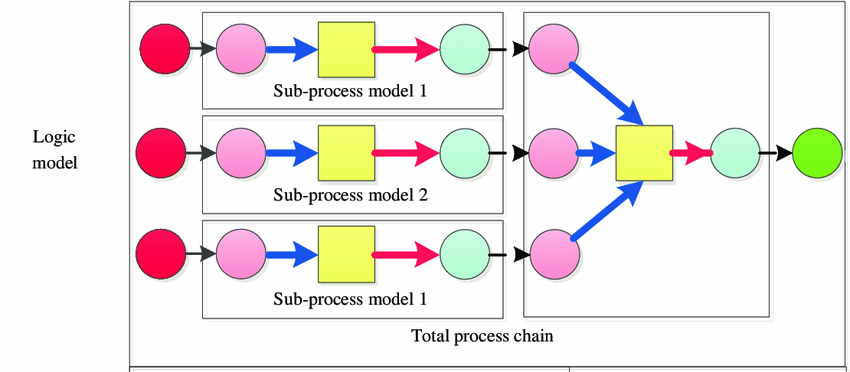
\includegraphics[width=0.8\textwidth]{logic.png}
	\caption{逻辑链中的“节点”是文本或图像上的关键信息,例如物体名称、类别、属性、关系等,“有向线段”表示“节点”间的逻辑关系}
	\label{logic}
\end{figure}

受神经网络在计算机视觉和自然语言处理成功应用的影响,从2014至今的视觉问答研究多采用了神经网络模型,使用卷积神经网络CNN提取图像特征,使用卷积神经网络RNN或者长短期记忆LSTM处理文本信息,再通过不同的方式“融合”图像特征和文本特征得出答案。这种架构在识别任务相关的问题上能有可接受的表现,但在复杂推理任务上就显得性能堪忧,如果问题中涉及图像以外的物体时,系统很难得到令人满意的答案,这是因为训练集的不完备导致的。因此在复杂推理任务的解决上,一方面可以通过不断完善数据集的方式,让系统在训练过程得到足够多的“经验”,另一方面可以为系统提供额外的知识库,让系统能在其知识网络搜索、游走,通过逻辑链条得到正确且有意义的答案。

本文将研究知识库在视觉问答上的应用情况,本章将简要介绍视觉问答几个重要的数据集和常见方法;第二章将重点介绍知识库与视觉问答相结合的已有成果;第三章关注如何评估系统在开放性问题和推理问题上的表现;第四张提出基于知识库的视觉问答未来将面临的挑战和发展方向。

\section{视觉问答的国内外研究历史与现状}
时域积分方程方法的研究始于上世纪60 年代,C.L.Bennet 等学者针对导体目
标的瞬态电磁散射问题提出了求解时域积分方程的时间步进(marching-on in-time,
MOT)算法。

\section{数据集}
从LeCun的MNIST数据集\citing{lecun1998mnist}到如今各式各样的计算机视觉等人工智能任务的数据集,优质的数据集已经成为了智能系统成长的“食粮”,尤其是神经网络复兴以来,计算机视觉和自然语言处理等任务的快速迭代蜕变一直都离不开数据的收集和整理工作\citing{deng2009imagenet,lin2014microsoft,rajpurkar2016squad}。关于数据更重要还是算法更重要的争论还继续,但数据集对于智能任务的训练价值是有目共睹的,当然,前提是数据集具有足够大的容量\citing{sun2017revisiting}、规范友好数据格式、较小的数据偏见等特点。视觉问答任务是在经历了计算机视觉和自然语言处理任务成功之后的新的颇具野心的构想——让系统能同时理解多模信息,并完成信息整合与推理。自从2014年以来,多个高质量的数据集为这个人工智能领域“新生儿”的快速成长提供了坚实的保障——DAQUAR\citing{malinowski2014multi}、COCO-QA\citing{ren2015exploring}、VQA\citing{antol2015vqa}、VQA 2.0\citing{goyal2017making}、CLEVR\citing{johnson2017clevr}、VQA-CP\citing{agrawal2018don}、KB-VQA\citing{wang2015explicit}。

\subsection{DAQUAR}
DAQUAR从NYU-Depth V2中带有语义分割标注的图片基础上扩展而来\citing{malinowski2014multi}。数据集包含1449张图片,图片多为室内场景,这大大地限制了数据集的场景丰富性,是该数据集的一大劣势。数据集由训练集和测试集两部分组成,训练集中包含6794对“问题-答案”,测试集中包含5674对“问题-答案”,“问题-答案”对由算法生成或是人类志愿者提供,算法生成的“问题-答案”对根据给定的模板生成,详见图\ref{DAQUAR}。

\begin{figure}[H]
	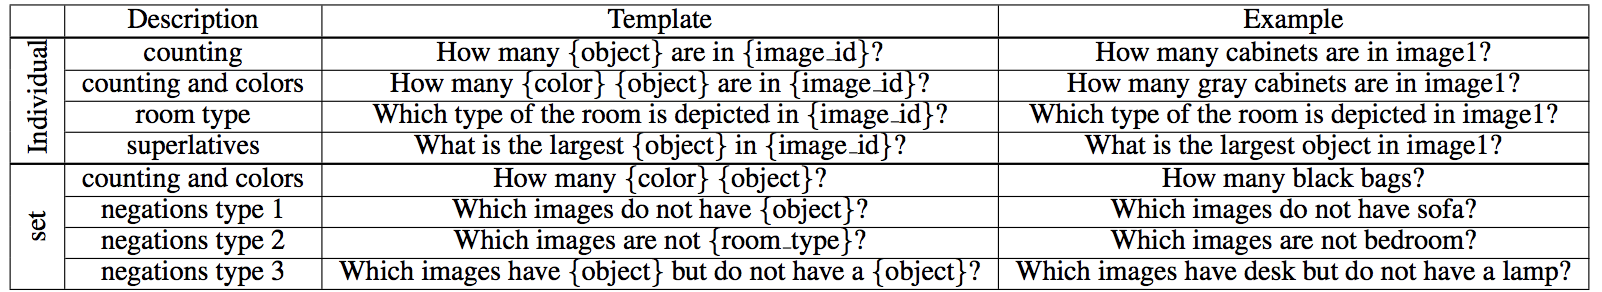
\includegraphics[width=0.8\textwidth]{DAQUAR.png}
	\caption{DAQUAR问题模板}
	\label{DAQUAR}
\end{figure}
DAQUAR数据集较小并且问题的类型只有三种:物体识别、色彩识别、计数,并且答案类型多以单词为主,因训练和测试系统复杂问题的推理能力较弱,偏于传统的物体识别任务。作为较早提出的针对视觉问答的数据集,为此后的数据集丰富工作提供了有益的方向。

\subsection{COCO-QA}
COCO-QA包含来自MS COCO的123287张真实场景图片,”问题-答案“对则是运用算法从MS COCO数据集的图片说明中生成的,为了方便生成算法的运用,将问题划分在物体识别、色彩识别、计数、地点查询四种类型。DAQUAR数据集在实际测试过程中,被发现仅仅通过简单的猜测答案的方式都能获得较高的正确率,这使得高准确率出现了极大的偏差,不能公正的测试系统的“推理”能力。为了克服该缺点,COCO-QA去除了出现频数极低和极高的一些答案,使得常见答案出现的评率从24.98\%下降到7.30\%。COCO-QA的训练集包含78736对“问题-答案”,测试集包含38948对“问题-答案”,在四个类别中的分布如图\ref{coco-vqa}。

\begin{figure}[H]
	\centering
	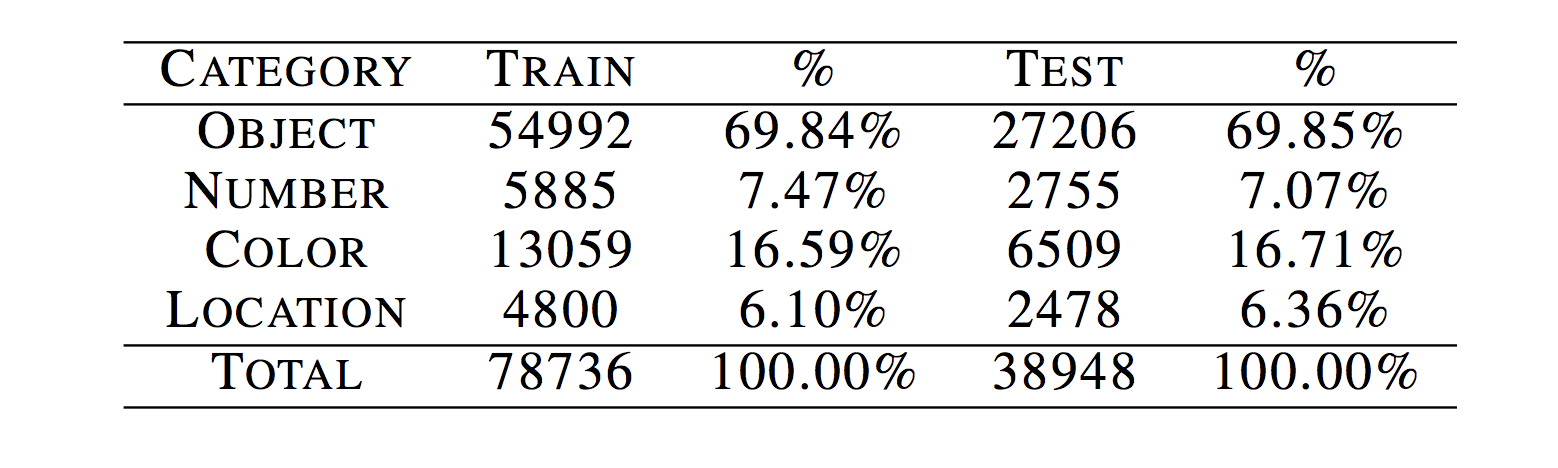
\includegraphics[width=0.8\textwidth]{coco-vqa.png}
	\caption{coco-vqa中“问题-答案”对的分布情况}
	\label{coco-vqa}
\end{figure}

\subsection{VQA}
VQA数据集是视觉问答领域发展的一个重要拐点,在此之前的数据集的问题类型被限制在一些模板之中,这使得数据集不能很好地测试出视觉问答系统在真实语境下的表现,例如,DAQUAR将答案仅仅限制在16种基本颜色和894种物体类别中\citing{malinowski2014multi}。VQA数据集中的问题和答案是无限制、开放式的,且全部由人类产生,同时图片的数量相较DAQUAR提高了两个数量级,到达254731张,极大的提高了数据集的容量。VQA数据集不仅包含从MS COCO\citing{lin2014microsoft}中提取的204721张真实场景的图片,还提供了50000张合成的抽象场景图(如图\ref{vqa-exmaple}),丰富了数据库场景的多样性,同时为高阶的场景推理和复杂空间推理提供了便利。

\begin{figure}[H]
	\centering
	\subfigure[真实场景图像实例]{
		\label{vqa-real}
		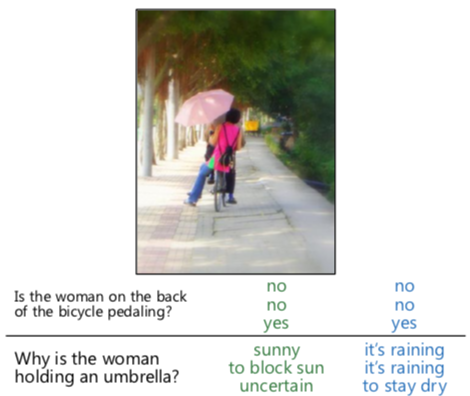
\includegraphics[width=0.4\textwidth]{VQA-real.png}}
	\subfigure[抽象场景图像实例]{
		\label{vqa-abs}
		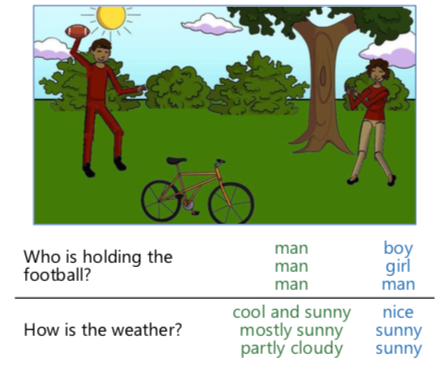
\includegraphics[width=0.4\textwidth]{VQA-abs.png}}
	\caption{VQA中的真实、抽象场景图像实例}
	\label{vqa-exmaple}
\end{figure}
为了实现对复杂推理的训练和测试,VQA数据集在问题设置上采用了人工的方式,每张图片都有3个人类提出的问题。答案则分为开放式和多项选择两种形式,开放式答案由于答案并不唯一,因此难以确定标准答案,因此正确答案的评估方法也引入人工评估机制:对于同一个开放性问题由十个人分别作答,如果有三个及以上的被测者均提供了同一答案,该答案被视为正确答案,这意味着同一个问题,可能会出现几个正确答案,这符合人类世界的真实状况,答案的不唯一性为训练智能系统多角度、多层次的“认知”提供了可能。多项选择的答案则由四种类型、18个候选项组成(如图\ref{vqa-multi}):
\begin{description}[labelindent=2em, leftmargin=6em, style=sameline]  
\item [正确答案] 一个,从被测者回答中取最为常见的作为正确答案
\item [混淆答案] 三个,不看图,仅根据问题作答的答案
\item [常见答案] 十个,数据集中最出现频数最高的十个答案
\item [随机答案] 四个,除去已经列出的选项,随机挑选四个答案
\end{description}
\begin{figure}[H]
	\centering
	\subfigure[真实场景图像的多选实例]{
		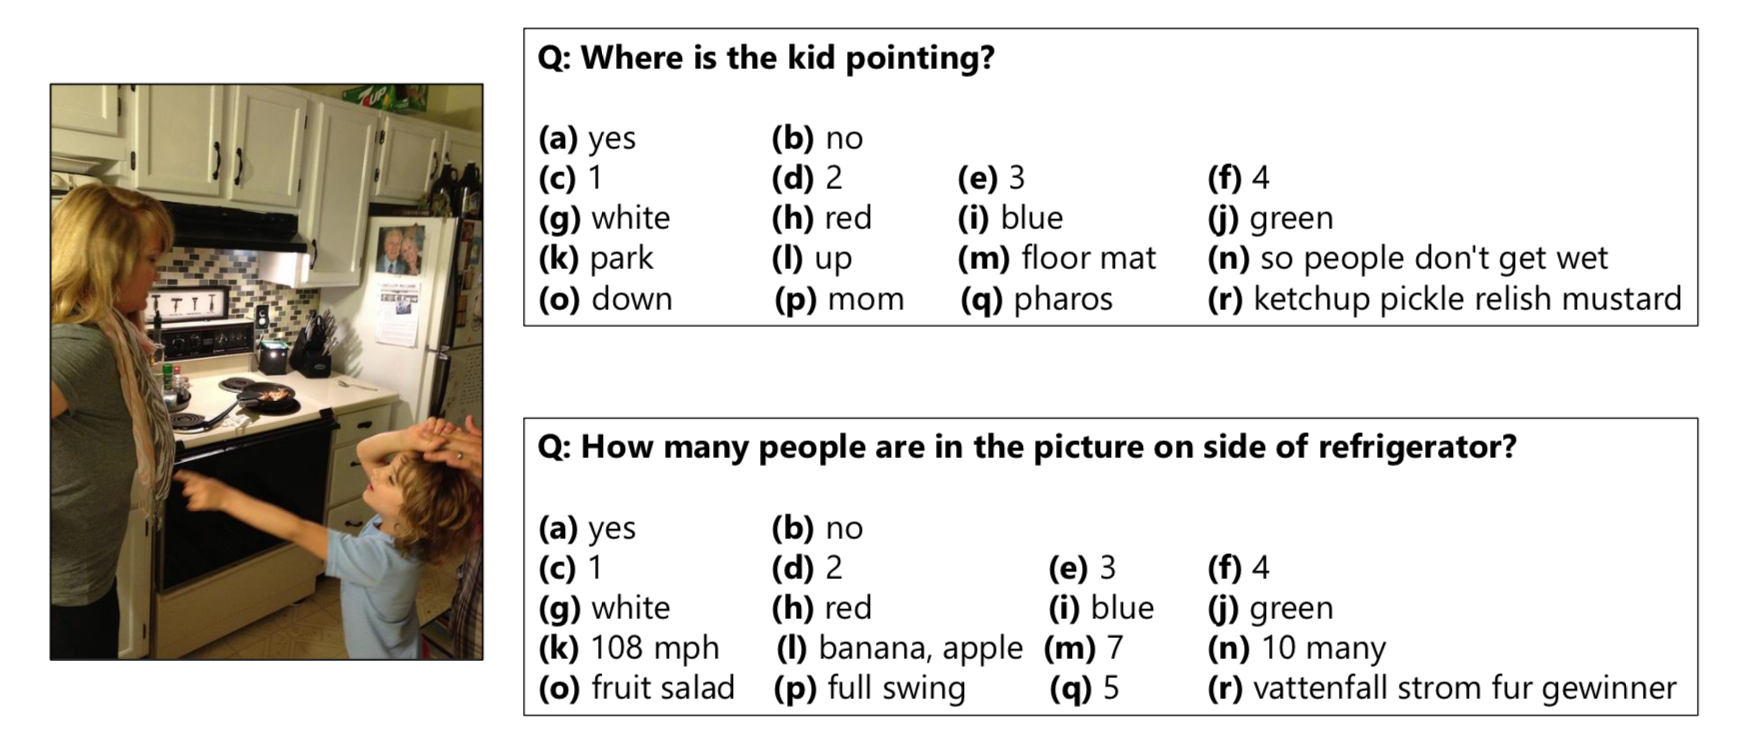
\includegraphics[width=0.8\textwidth]{vqa-multi.png}}
	\subfigure[抽象场景图像的多选实例]{
		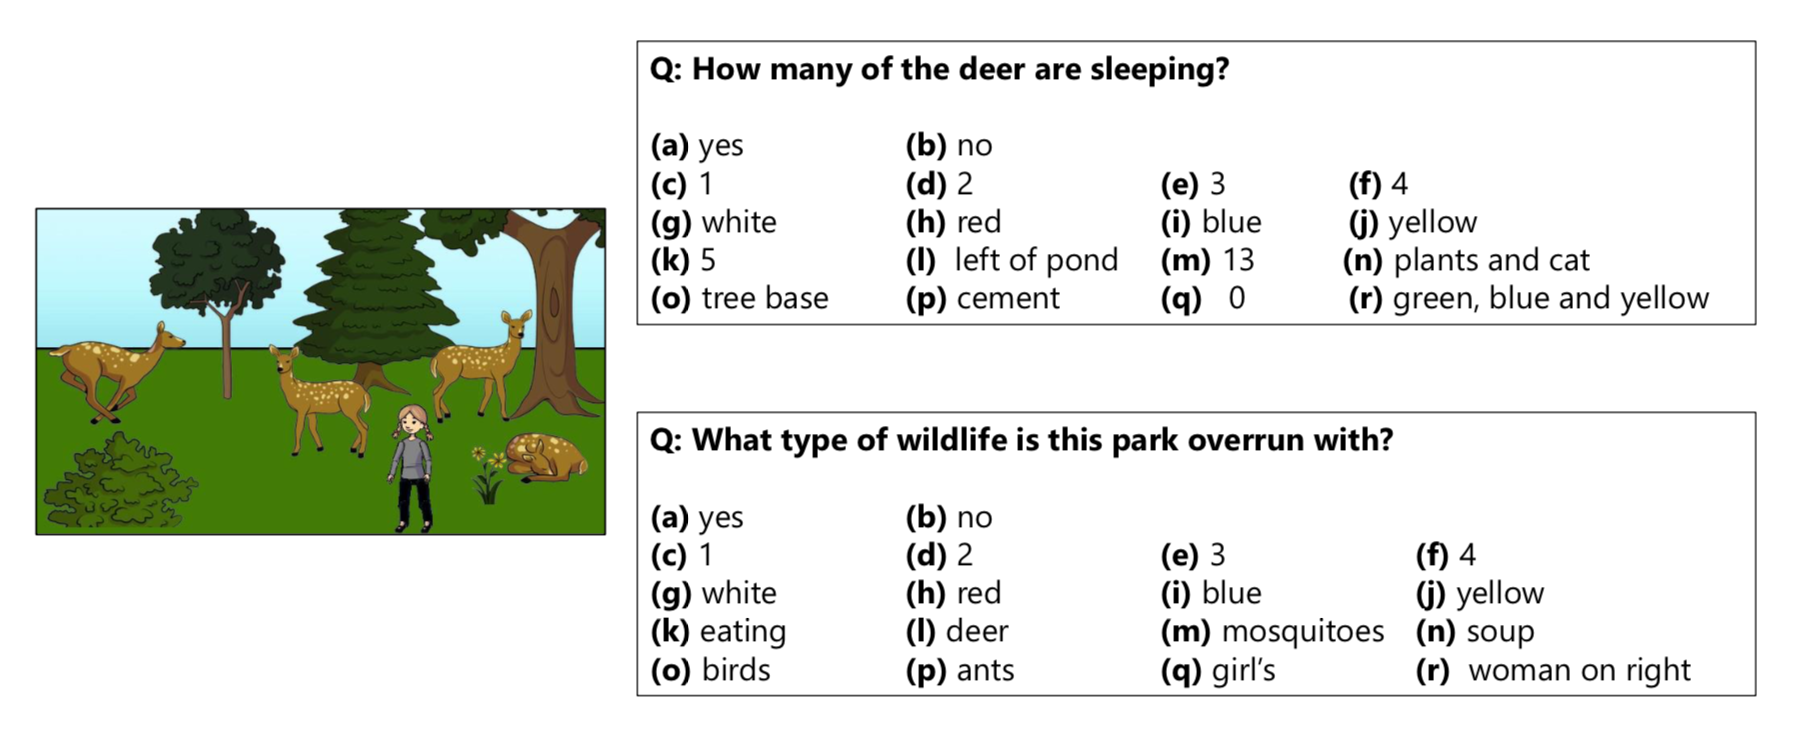
\includegraphics[width=0.8\textwidth]{vqa-multi2.png}}
	\caption{VQA中的真实和抽象场景图像的多项选择实例}
	\label{vqa-multi}
\end{figure}

\subsection{VQA 2.0}
VQA数据集由于其建立了开放性问题和多项选择问题的评测标准受到了许多研究者的追捧,成为众多算法的测试数据集,但VQA数据集中的语言偏见问题也受到了研究人员的察觉和诟病。正是由于语言偏见的问题,即使是完全无视图像的算法也能在VQA数据集上得到49.6\%的准确率\citing{ren2015exploring},这意味在VQA数据集的测试环境下,系统对于视觉信息的需求程度远远小于语言信息,这种状况相较于人类对于图像问答任务中的真实体验而言,是严重不符的。例如,答案为”是或否“的问题占所有问题的38\%,并且大约59\%的二值问题答案都为”是“;询问”什么运动“的问题中有41\%的答案为”网球;询问数量的问题中有39\%的答案为“2”。

针对以上问题,VQA 2.0应运而生。VQA 2.0通过在原有的VQA数据集基础上补充新的“混淆数据”实现数据集对视觉信息的增强。“混淆数据”和原始数据一样由(图像I,问题Q,答案A)的形式组织,不同的是新补充的图像与原有图像相似,但回答同样的问题Q却得到不同的答案A(如图\ref{vqa2})。针对同样的问题,在不同图片背景下需要得到不同的答案,这要求系统不仅能理解自然语言问题,同样需要关注图片的语义差异,才能得到正确的答案,这种平衡的方法能够筛选掉弱化图像理解的算法,强化了图像理解在视觉问答任务的重要性。补充后的VQA 2.0包含110万对”图像-问题“、20万张关联1300百万个问题的真实场景图片,数据量几乎是VQA数据集的两倍,势必会取代VQA数据集成为开放性问题的新测试标准。
\begin{figure}[H]
	\centering
	\subfigure[]{
		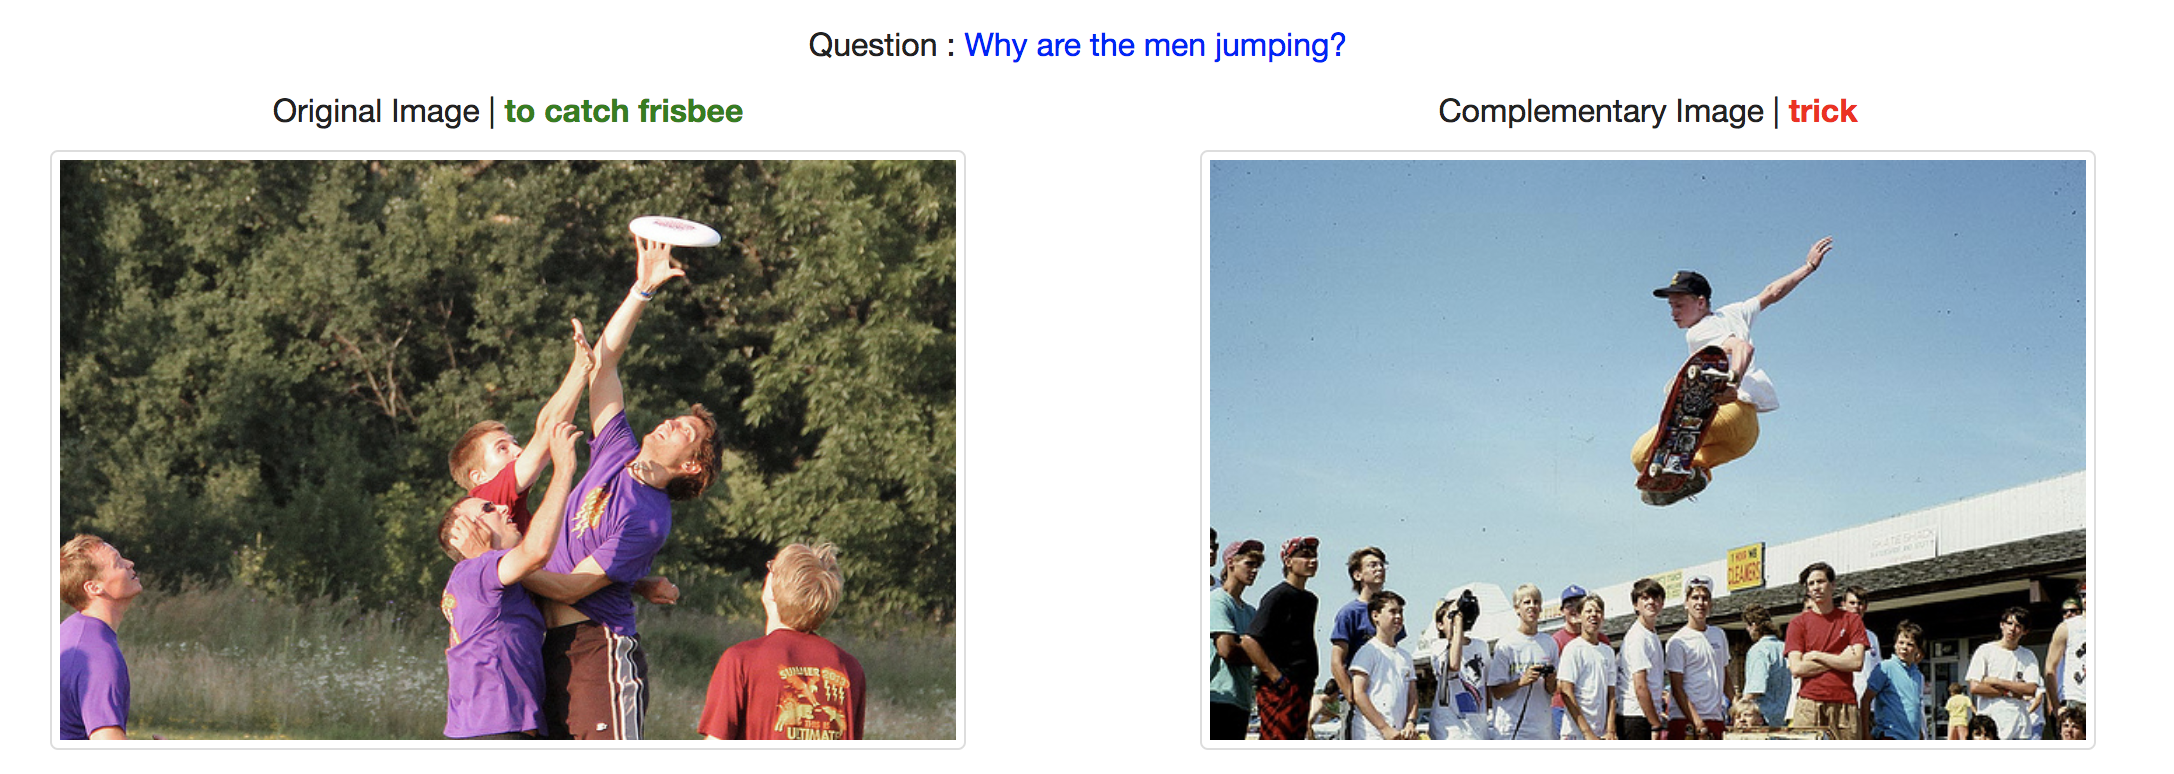
\includegraphics[width=0.8\textwidth]{vqa2-1.png}}
	\subfigure[]{
		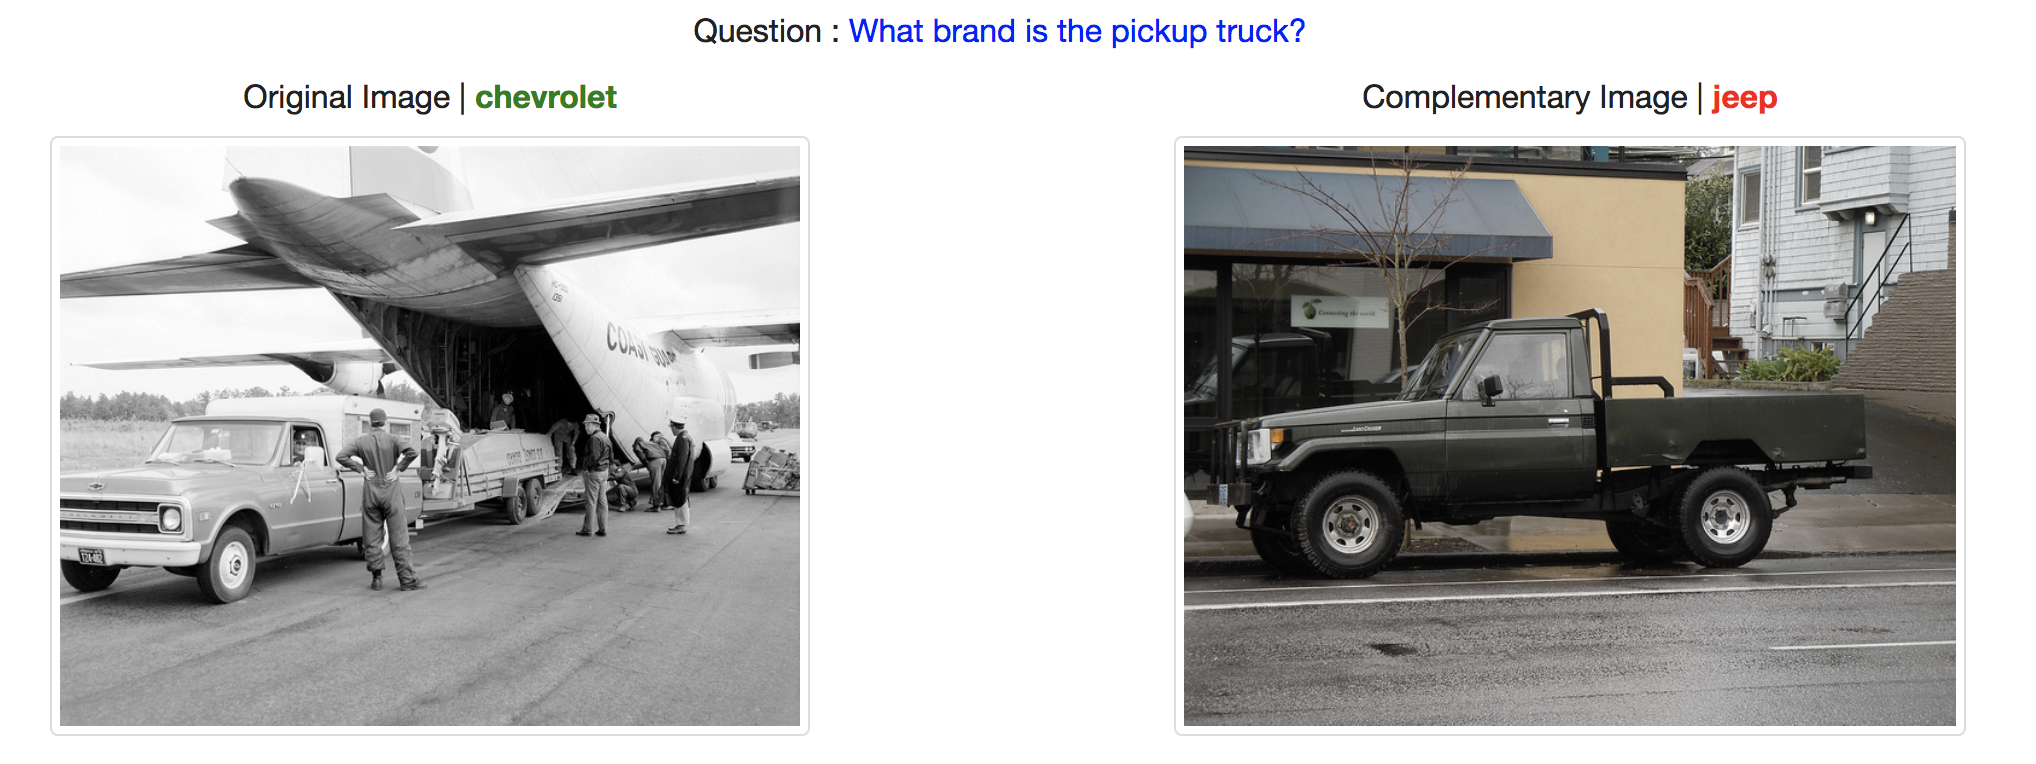
\includegraphics[width=0.8\textwidth]{vqa2-2.png}}
	\caption{VQA 2.0中针对同一问题的不同图像和答案实例}
	\label{vqa2}
\end{figure}

\subsection{CLEVR}
为了更加准确地衡量视觉问答系统各个方面的推理能力,Johnson等人提出了一个结合语言和基本视觉推理诊断数据集CLEVR。CLEVR包含10万张由空间立方体组成的合成图像、将近100万个问题,其中包含85.3万个独特的问题。在图像的设置上,CLEVR为了减小识别难度,关注系统的视觉推理能力,采用了由空间立方体组成的合成图像,并且每张图像均有包含所有物体位置和属性的说明(如图\ref{clevr})。CLEVR的问题也均由程序生成得到,涉及属性识别、计数、比较、逻辑运算等子任务。

为了减少问题的偏见,数据集生成的问题中有85\%是独特的;为了控制问题的准确性,数据集剔除了有歧义的问题,例如,询问“正方体右边的球体是什么颜色?”时,如果“正方体”右边有多个“球体”,问题便产生歧义,答案变得不唯一,使得评估过程变得复杂和不准确;为了保持问题的复杂性,数据集拒绝了一些看似复杂但实际上限定条件无效的问题,例如,询问“球体前面的圆柱体是否为金属的?”时,如果场景中仅有一个“圆柱体”,那么问题中的“球体前面”的限定便可以被忽略,这种情况降低了问题的复杂性。

由于CLEVR数据集对图像和问题具有完全的掌控,能实现其他数据集难以实现的能力测试,要求系统具有短期的记忆力、注意力机制、组合推理能力。
但同样因为其简单的图像场景设置,CLEVR不能测试出视觉问答系统在常识推理、复杂推理的表现,并且也不能衡量系统在真实场景中的识别能力和稳定性。
\begin{figure}[H]
	\centering
	\subfigure[尺寸、形状、样色、材质的标注]{
		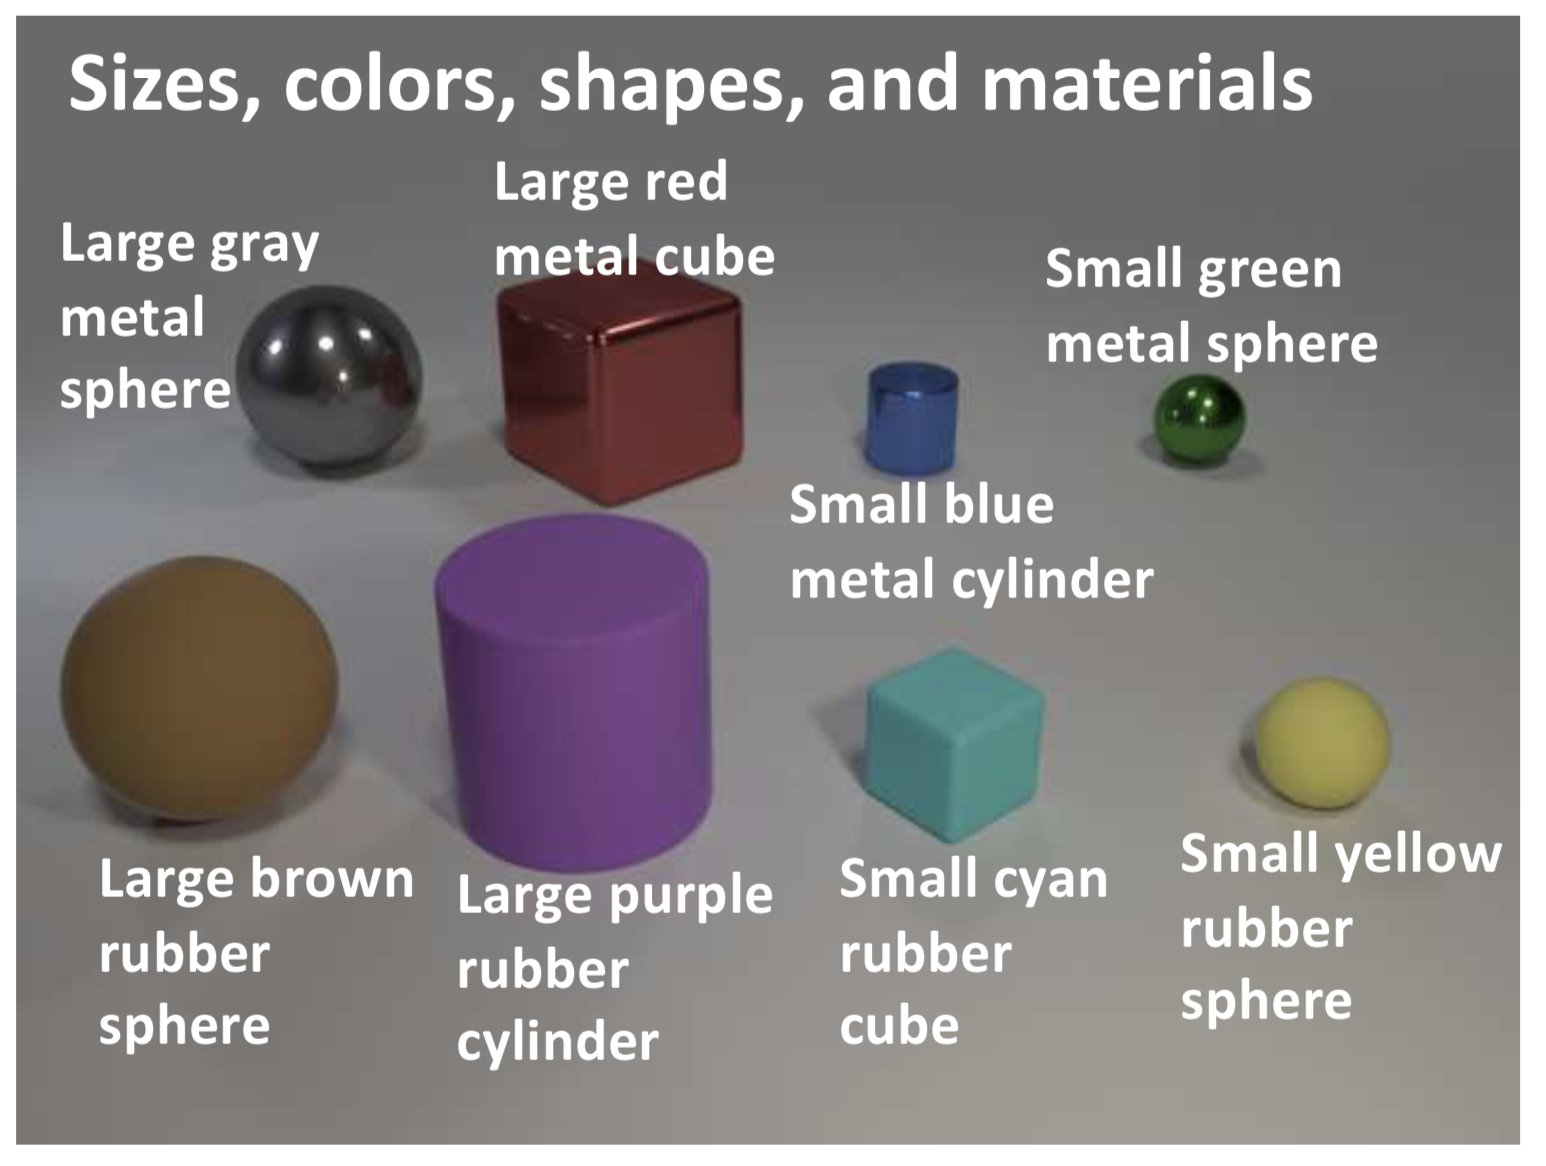
\includegraphics[width=0.3\textwidth]{clevr1.png}}
	\subfigure[空间左右的标注]{
		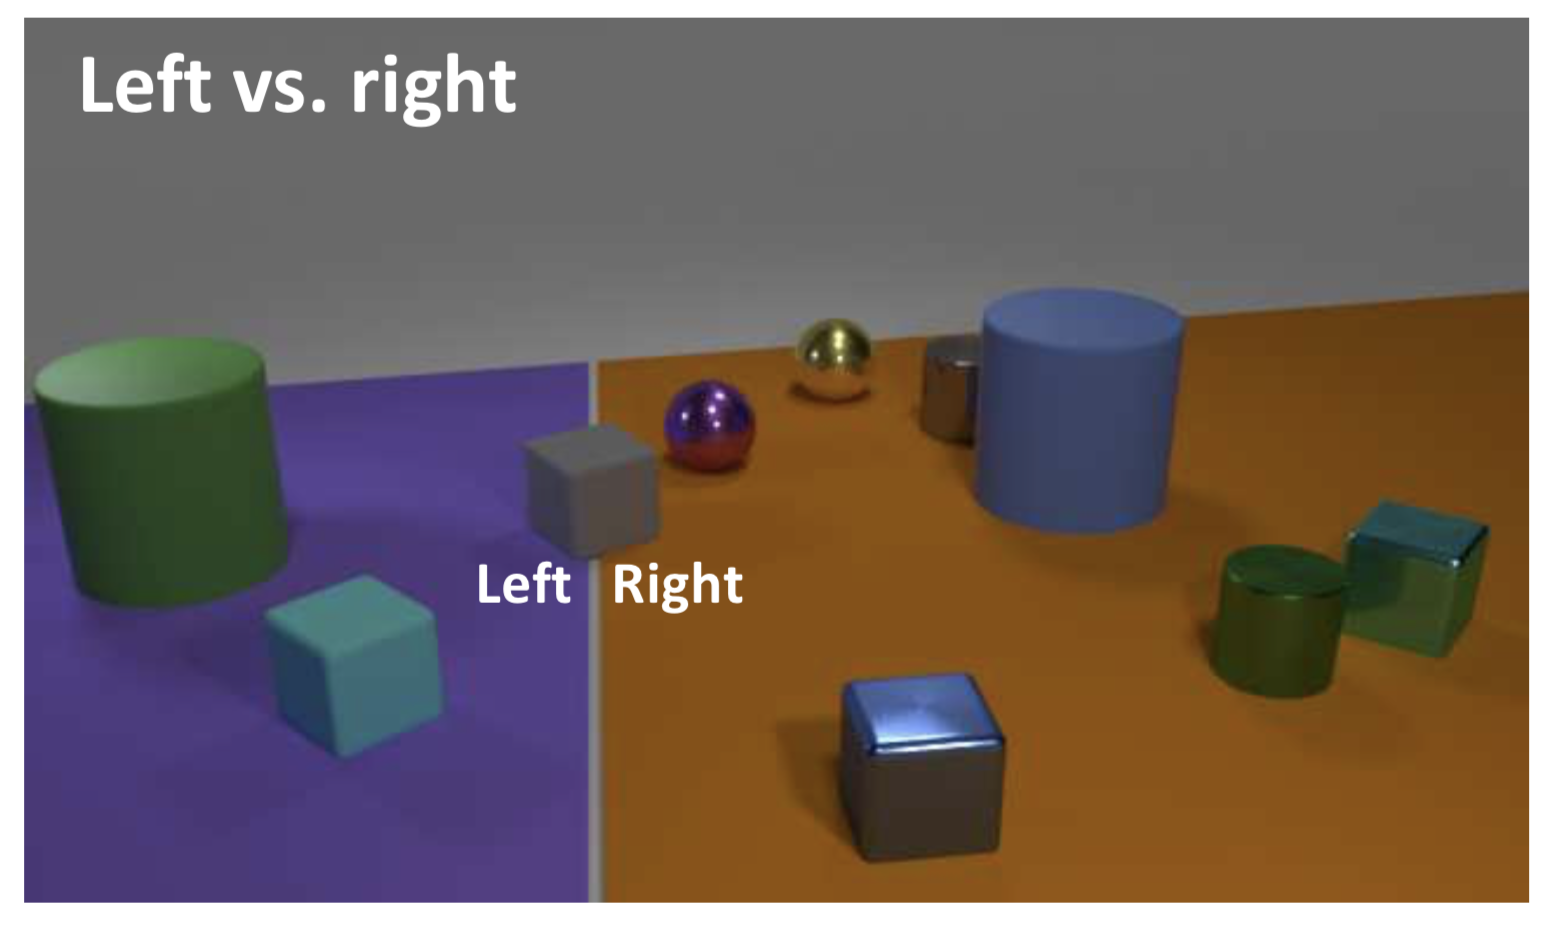
\includegraphics[width=0.3\textwidth]{clevr2.png}}
	\subfigure[空间前后的标注]{
		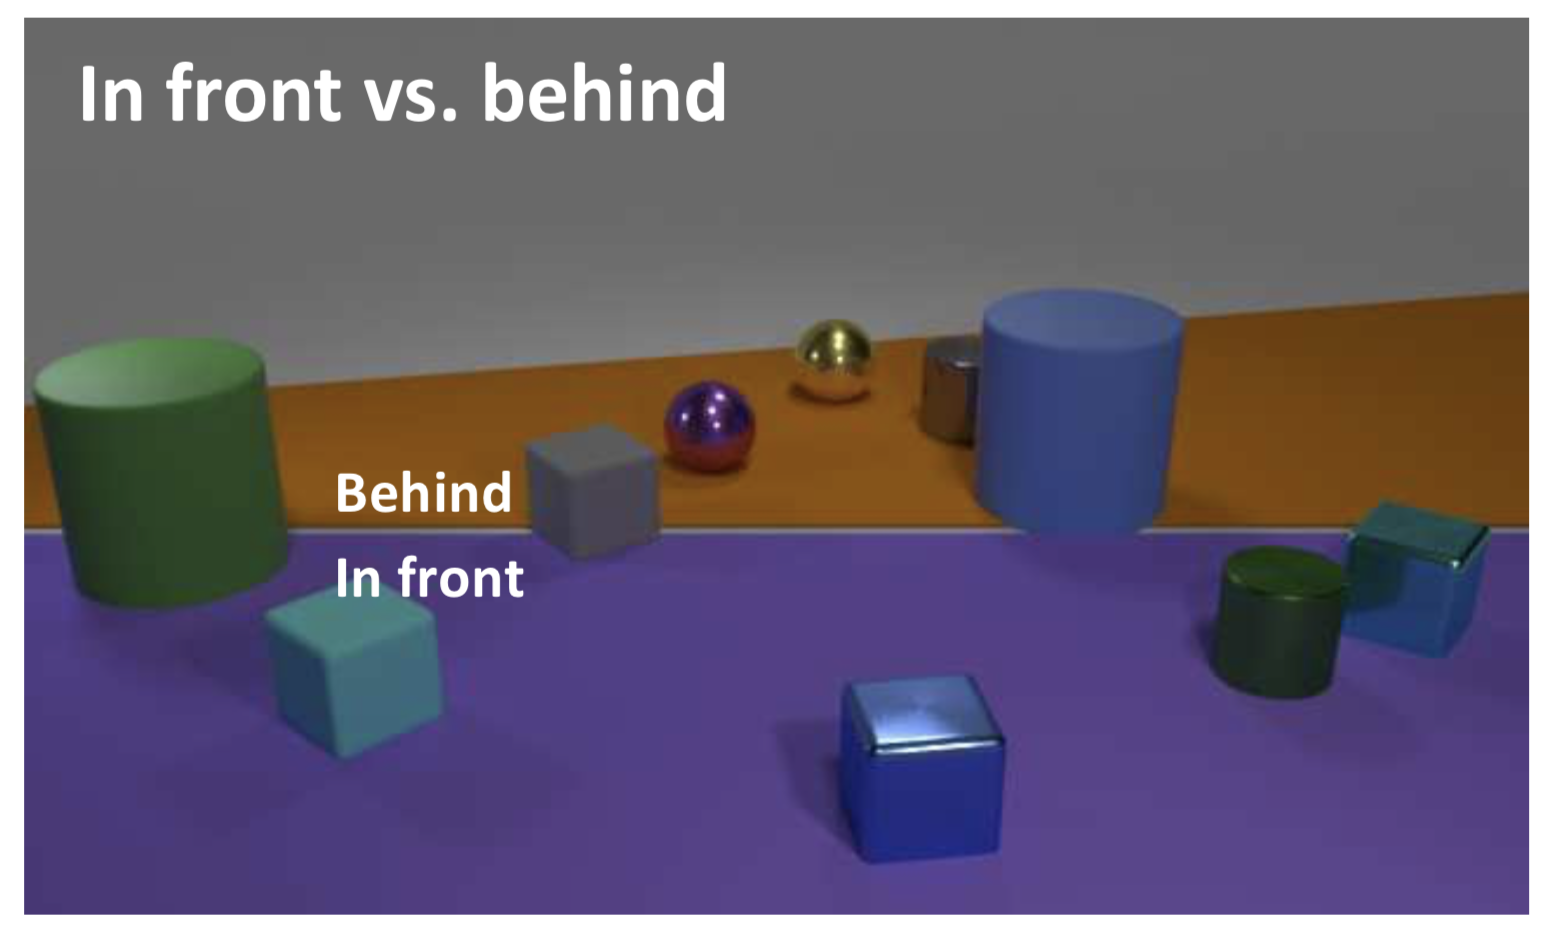
\includegraphics[width=0.3\textwidth]{clevr3.png}}
	\caption{CLEVR中图像标注}
	\label{clevr}
\end{figure}

\subsection{VQA-CP}
数据集一般会划分为训练集和测试集两个部分,在视觉问答任务中同样如此。如果训练集中的答案分布存在偏见,且测试集与训练集之间的答案分布相近,那么系统便可以通过记忆在训练过程中得到的数据偏见,并将其应用于测试过程,这样得到的准确率的可信度将会打折扣,例如,在训练集中询问颜色的问题中“白色”最为常见,同样在测试集中的“白色”也为热门答案,这回干扰系统的评估结果,不清楚系统是通过正确推理得到还是”经验“得到的。

针对训练集和测试集中问题答案分布相似的状况,VQA-CP重新对VQA数据集和VQA 2.0进行划分,重新划分得到的训练集和测试集在每个问题类型中的答案分布均不同,例如,在训练集中询问颜色的问题中,“白色”、“红色”为最常见的答案,而在测试集中“黑色”、“粉色”为最常见的答案;对于询问运动类型的问题,在训练集中“网球”为最多的答案,而在测试集中“滑雪”为最常见的答案(如图\ref{vqa-cp})。
\begin{figure}[H]
	\centering
	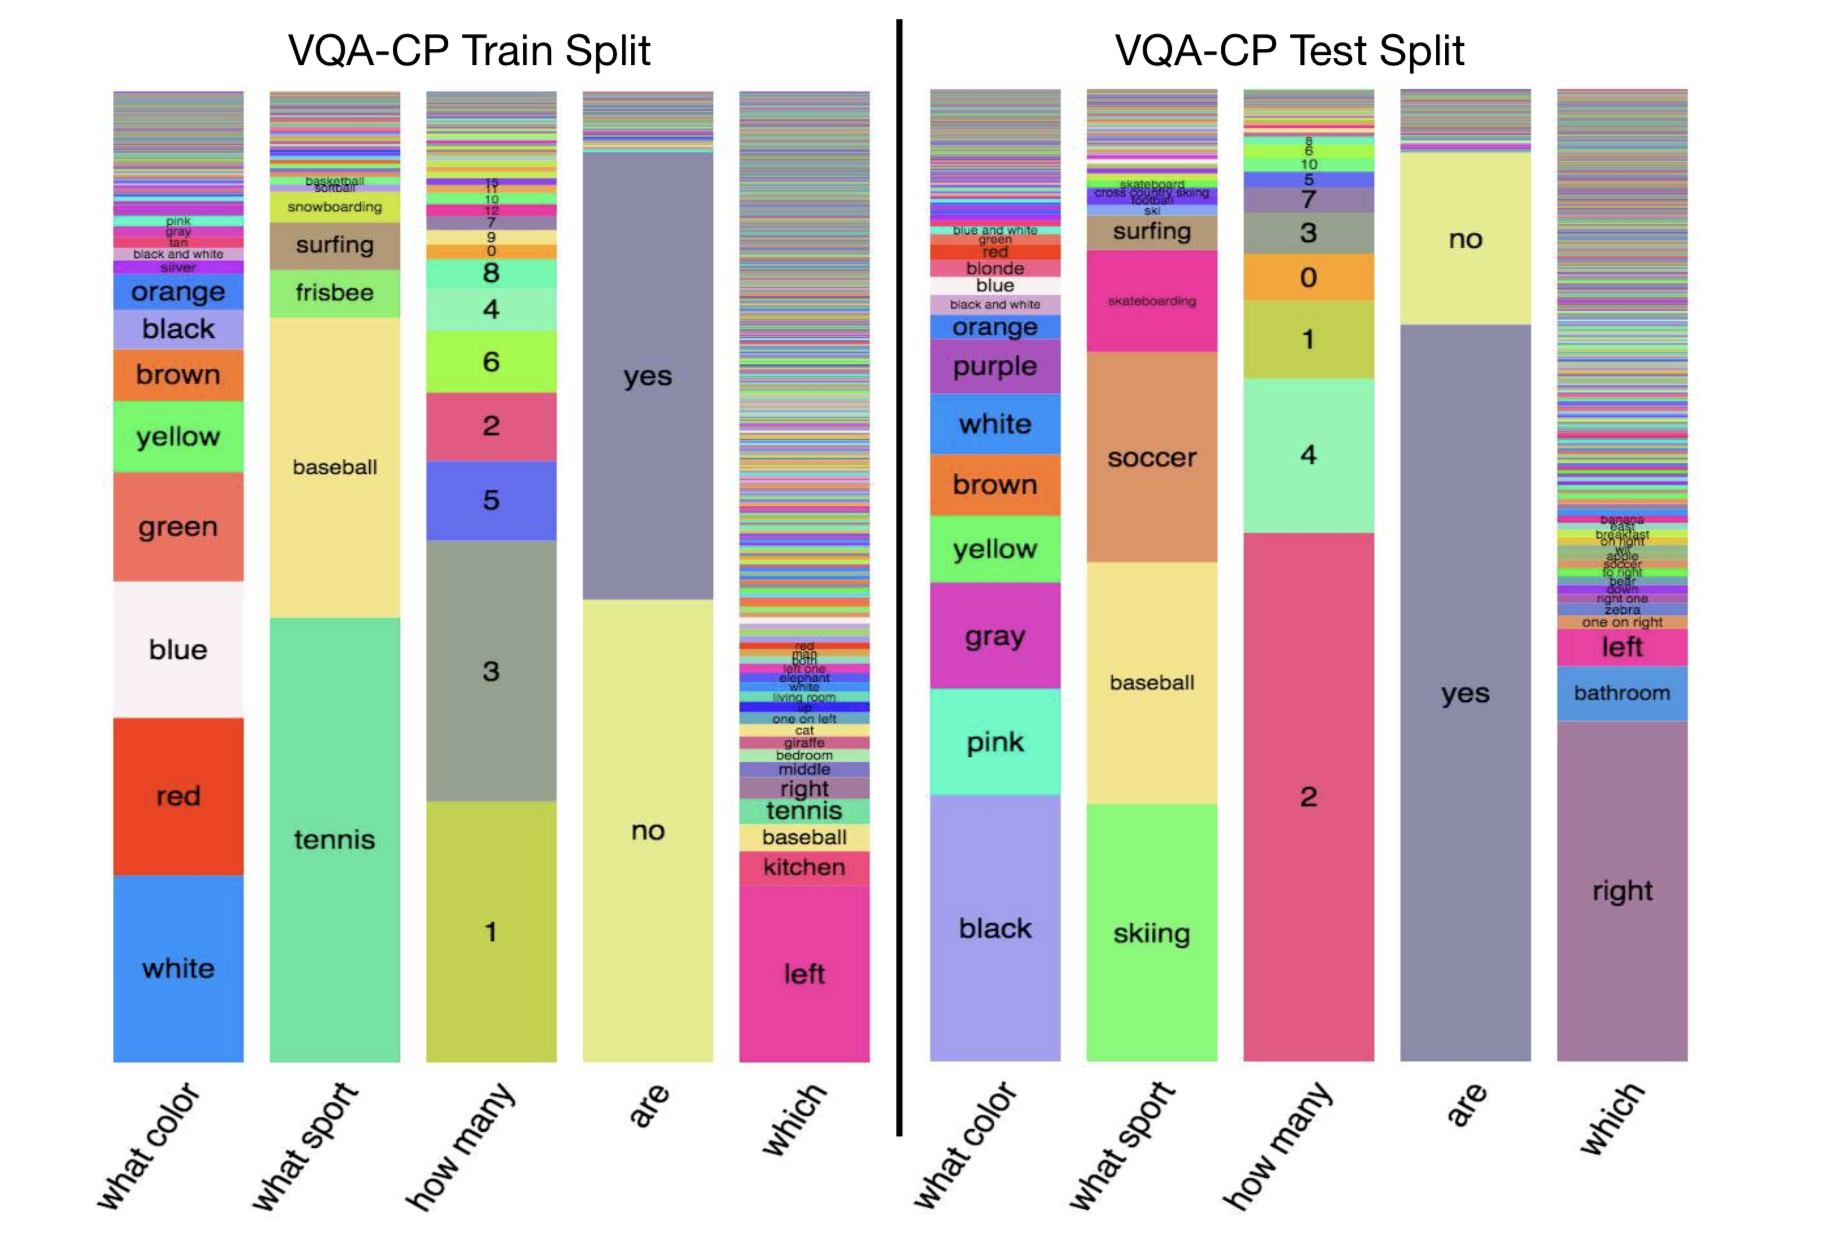
\includegraphics[width=5in]{vqa-cp.png}
	\caption{vqa-cp训练集和测试集的答案分布}
	\label{vqa-cp}
\end{figure}

\subsection{KB-VQA}
回答VQA等数据集中的开放性问题可能涉及常识或者特定领域知识的先验知识,但已有数据集中还掺杂着大量不需要先验知识的训练样本,因此为了更好的评估VQA算法对需要高层次知识问题的准确推理能力,Wang等人构建了只包含复杂推理问题的数据集KB-VQA\citing{wang2015explicit}。

KB-VQA数据集从MS COCO\citing{lin2014microsoft}中挑选出700张图片样本,挑选出的图片包含150个物体类别和100个场景类别。每张图片附带有3-5个由人工生成的“问题-答案”对,所有的问题被限定在23种问题模板中,例如,“图片中是否存在某种概念?”,“图片中的某个物体被生产于什么地方?”等,详见\ref{qt}。

为了准确评估系统在需要先验知识的问题的表现,KB-VQA人工地赋予每个问题一个表示所需不同知识类型的标签,“视觉问题”、“常识问题”和“知识库问题”,其中“视觉问题”表示仅仅从图片中便可以获得答案的问题,例如,“物体是否存在于图片?”、“列出图片中包含的所有事物?”等,“常识问题”需要结合成人级别的常识和图像内容得出答案,例如,“图片涉及什么场景?”,“知识库问题”则需要某个领域特定的知识才能完成作答,例如,“图中的物品在哪一年被发明?”。23种问题模板在不同问题标签的分布如图\ref{qtd}。
\begin{figure}[H]
	\centering
	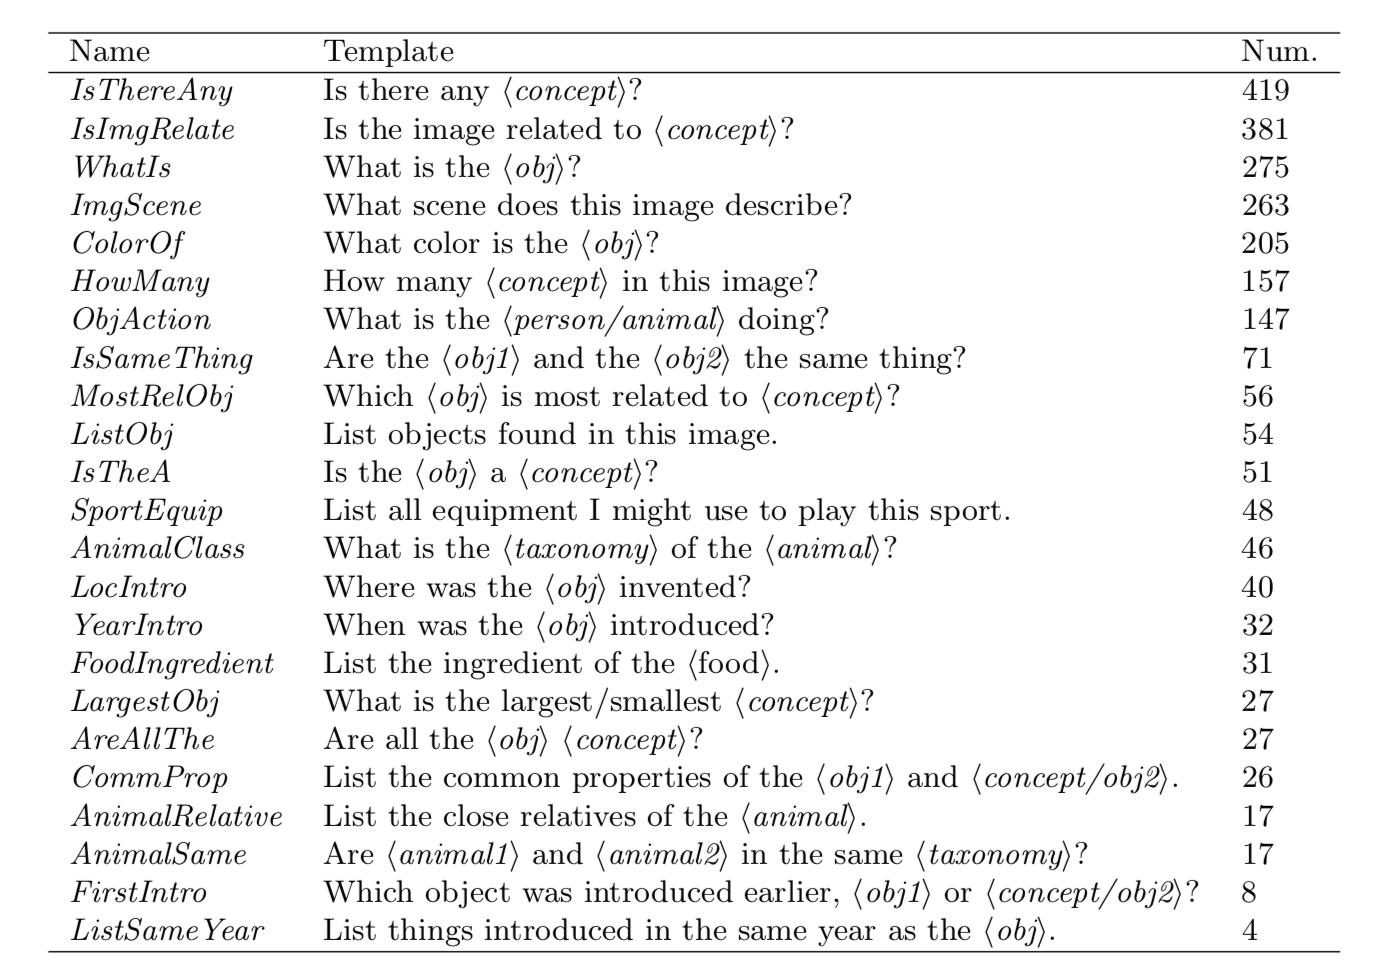
\includegraphics[width=0.8\textwidth]{qt.png}
	\caption{KB-VQA中23中问题模板及对应的问题数量}
	\label{qt}
\end{figure}
\begin{figure}[H]
	\centering
	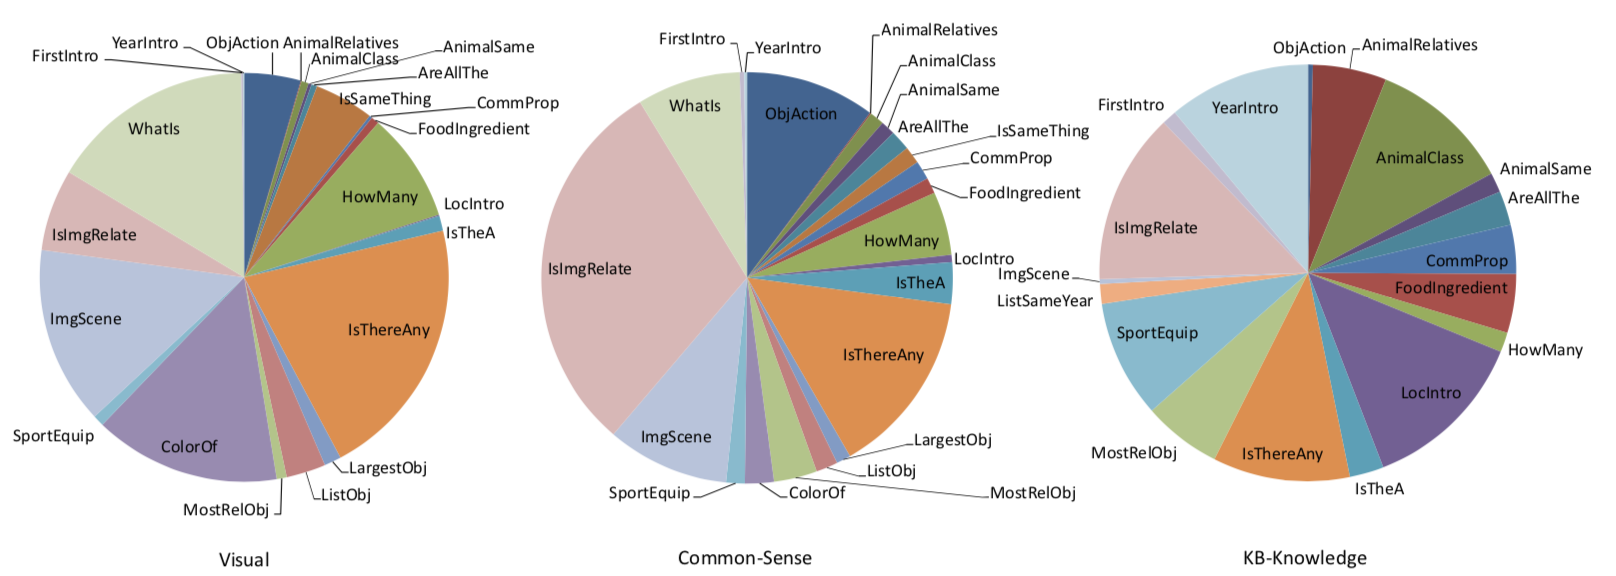
\includegraphics[width=0.8\textwidth]{qtd.png}
	\caption{KB-VQA中23中问题模板对应“视觉问题”、“常识问题”和“知识库问题”的分布情况}
	\label{qtd}
\end{figure}

数据集中的“视觉问题”、“常识问题”和“知识库问题”数量分别是1256、883和263,就图片和问题的数量而言,KB-VQA数据集相较于COCO-QA等数据集是非常小的,而且从图\ref{qt}也容易看出,有16种问题类型的问题数量都不超过100个,甚至有个位数的问题数量,数据集的不均衡和小容量很难准确得评估出系统在细分问题类型上的推理能力。但需要先验知识的问题占比要远高于大型数据集,DAQUAR\citing{malinowski2014multi}几乎全是“视觉问题”,COCO-VQA\citing{ren2015exploring}仅仅包含5.5\%的问题需要常识,没有问题需要额外的知识库。

KB-VQA在评估系统的复杂推理能力方面提供了一个解决方案,但数据集的容量、平衡性和多样性方面还需要更多的丰富,并且随着数据集的扩充,自动化和标准化的评估方式也相应的需要完善。

\subsection{FVQA}
为了评估视觉问答系统在需要先验知识的问题上的表现,Wang等人提出了FVQA数据集\citing{wang2017fvqa}。回答FVQA中的问题需要额外的知识,但不同于一般的数据集,FVQA将(图片,问题,答案)的三元组数据扩展为(图片,问题,答案,支持事实)的四元组形式,其中“支持事实”是回答问题所需要的额外知识,使用资源描述框架(RDF)的三元组形式,例如(猫,可以,爬树)。

FVQA从MS COCO\citing{lin2014microsoft}和ImageNet\citing{deng2009imagenet}中挑选出1906张图片,并对图片预处理,提取出三种类型的视觉概念:物体对象、场景和行为,最终提取出326种物体对象、21种场景和24种行为。为了获取与视觉概念相关的知识,FVQA以DBpedia\citing{auer2007dbpedia}、ConceptNet\citing{liu2004conceptnet}和WebChild\citing{tandon2014webchild}为知识源,从三种知识库中与视觉概念相关的所有知识中筛选出包含12种常见的谓语的知识,例如,关于分类的知识——“目录属于”、关于地点的知识——“地点所在”、关于大小比较的知识——“体积大于”,详见图\ref{fvqa_vc}。提取的知识以资源描述框架(RDF)的形式存储作为“支持事实”。
\begin{figure}[H]
	\centering
	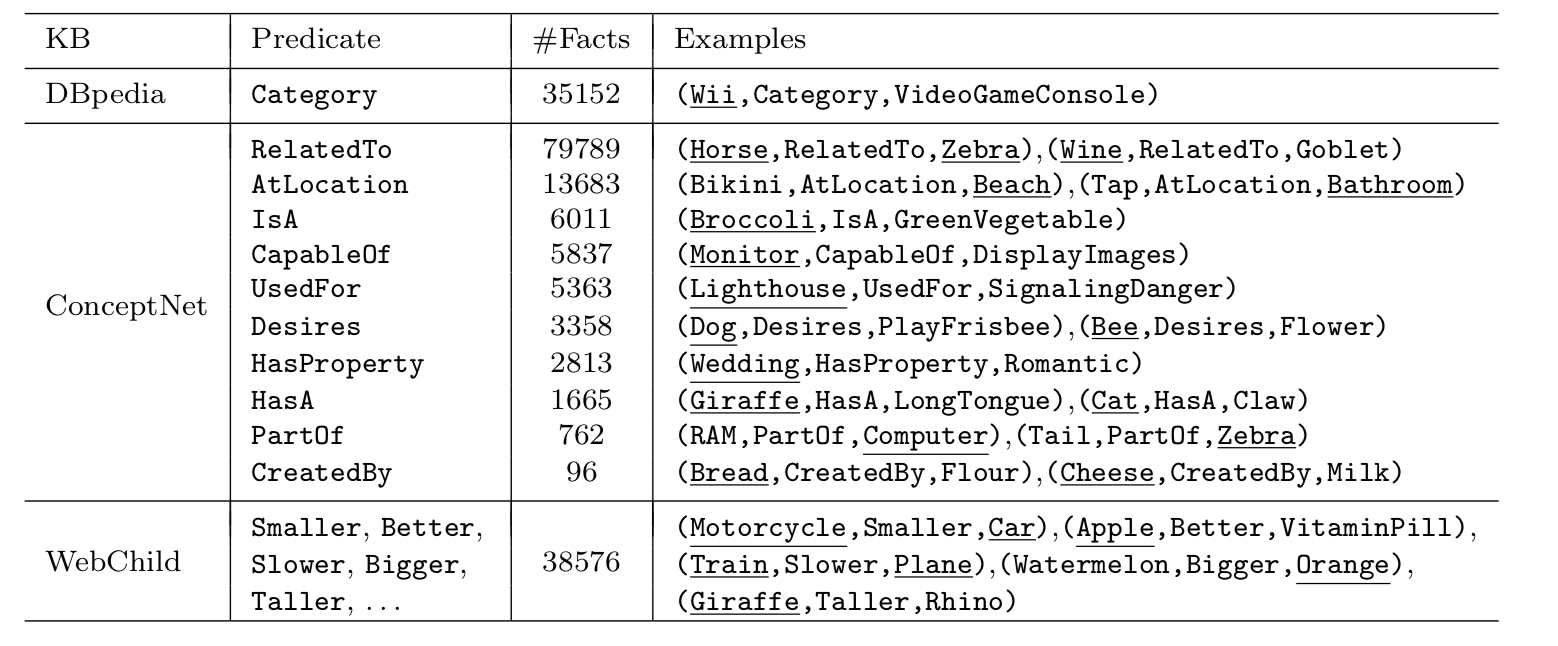
\includegraphics[width=0.8\textwidth]{fvqa_vc.png}
	\caption{从三种知识库中提取的知识涉及的12种谓语及相应的数量}
	\label{fvqa_vc}
\end{figure}

FVQA的问题和答案均使用人工的方式收集得到,被试者先选择图片中的一个视觉概念和一个与视觉概念相关的支持事实,再根据视觉概念和支持事实给出问题和答案,答案的来源要么是图片中的视觉概念要么是支持事实中涉及的概念。数据集最终包含4608个需要先验知识的问题,涉及3458条事实。根据视觉概念的类型,这些问题可以归为物体对象、场景和行为三种类型;根据支持事实的来源,可以归为DBpedia、ConceptNet和WebChild三种类型;根据答案来源,可以归为图片来源和知识库来源两种类型,不同分类在训练集和测试集的数量分布如图\ref{fvqa_cd}。
\begin{figure}[H]
	\centering
	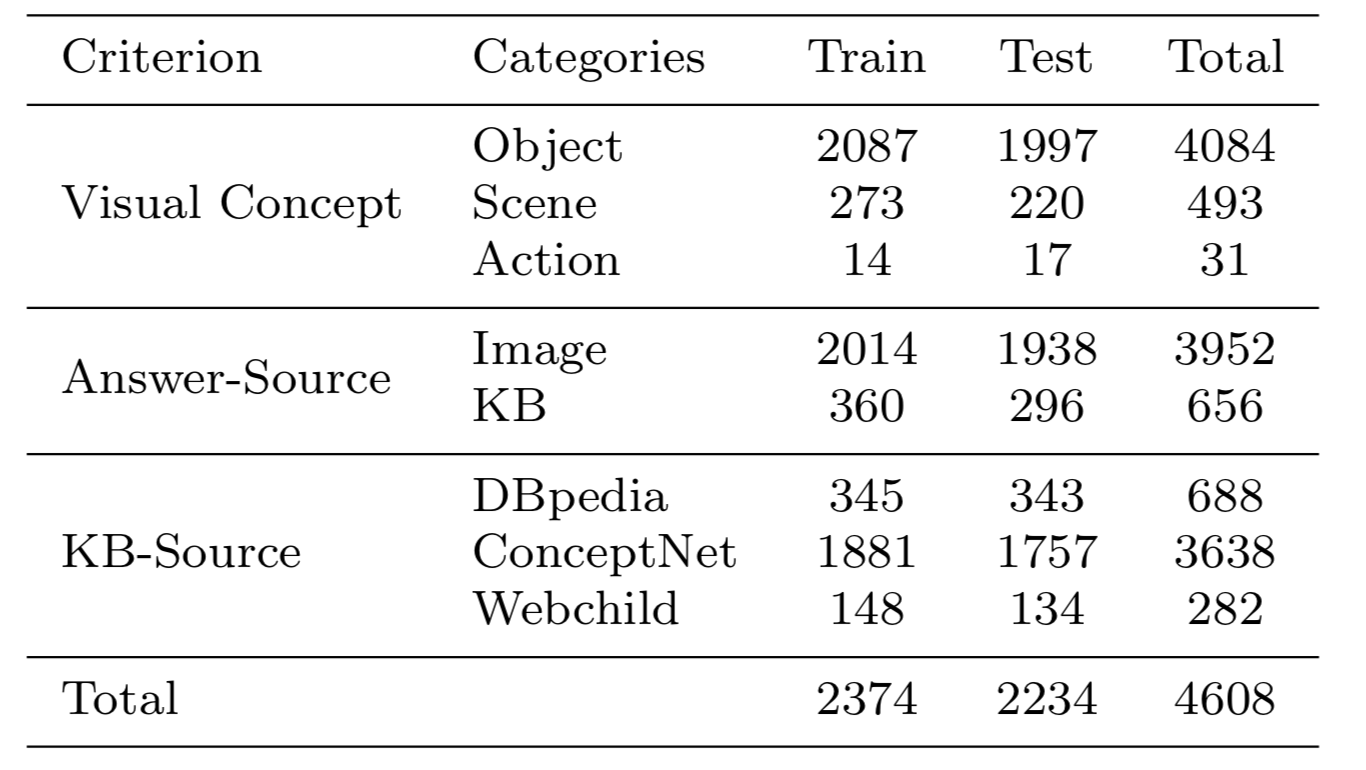
\includegraphics[width=0.8\textwidth]{fvqa_cd.png}
	\caption{不同分类在训练集和测试集的数量分布}
	\label{fvqa_cd}
\end{figure}

从统计的数据上不难看出,绝大多数问题是针对图像中的物体对象,这与提供的视觉概念中物体对象的高占比有强关联,从知识来源上分析,答案除了能从图像中获得外,还包含14\%的答案需要从额外知识库中获得,并且问题中不包含“是或否”的二值问题,这降低了系统”猜中正确答案“的情况。

FVQA和同样包含先验知识的数据集KB-VQA两者都能通过查询语言获取知识库中的数据,但不同于KB-VQA,FVQA拥更多的图片和问题数量,并且所有问题都需要额外知识。FVQA增加了ConceptNet和WebChild作为知识源,提高了知识库的多样性,能回答更多类型的问题,而不用预先设定问题模板。但FVQA数据集中几乎所有的答案都是物体对象,且为单个词语,不能训练模型给出对象关系的答案。FVQA数据集的支持事实多为单一谓语的句子,句式结构简单,如果用做训练集,不能考察模型应对多动词结构问题时的答案正确率。

然而两个数据集都面临着同样的问题:数据量的扩充和问题类型的扩充。两个数据集的问题收集都是通过人工的方式,并且参与者数量有限,因此直接导致了问题数量远低于其他自动化方法生成的数据集。大规模的协同工作和探索更多自动化方法是扩充数据集容量的方向。两个数据集都受到问题类型的限制,KB-VQA使用预先设定的问题模板,限制了问题的开放程度,FVQA虽然没有使用预先设定的问题模板,但其筛选的12种谓语间接的限制了问题的类型。扩展问题类型意味着额外知识库的扩充,也对视觉问答系统的问题解析提出了更高的要求,但这也能大幅的提高系统面对复杂多样的问题的开放性和鲁棒性。
\section{视觉问答方法}

视觉问答任务要求系统能同时正确理解问题文本内容和图像内容,一般而言视觉问答系统分为三个主要模块,a)从问题文本中提取特征,使得特征中包含足够多的语义信息。b)从图像中提取特征,理解图像中的物体信息、场景信息、活动信息、空间构成信息、颜色信息,将像素信息转化为系统可计算的数值量或者标签。 c)采用某种方式整合文本特征和图像特征,为系统建立一条高泛化能力、高稳健性、高准确率的答案生成通路。简而言之,视觉问答系统会图形和问题文本中分别提取特征,再将两者融合,最终以置信度高的候选答案作为输出(如图\ref{answer-generation})。

从视觉问答的处理过程可以看出,算法的核心有三个部分组成:如何提取出高层次的图像特征,例如,物体、属性、场景等;如何挖掘问题文本中的语义信息,以求能深入的理解问题内容,确定答案的形式和内容;如何结合图像特征和文本特征,得出正确或是最佳答案。图像特征提取的方法都来自于计算机视觉的已有成果,一般使用预处理后的卷积神经网络,例如VGGNet\citing{simonyan2014very}、 ResNet\citing{he2016deep}和GoogLeNet\citing{Szegedy_2015_CVPR}。问题文本的特征提取则借鉴了自然语言处理中的成果,例如词袋模型(BOW)\citing{zhou2015simple}、长短期记忆(LSTM)\citing{malinowski2015ask}、门控复发单位(GRU)\citing{noh2016image,kumar2016ask,xiong2016dynamic}。系统输出答案的方式有两种(如图\ref{answer-generation}),最常见的方式是将任务视为分类问题,根据候选项的概率大小,确定答案。第二种方式则直接由系统遣词造句合成答案语句,此类方法多出现在有额外知识库的视觉问答系统中,例如Attributes-LSTM\citing{wu2016value}、ACK\citing{wu2016ask}、Ahab\citing{wang2015explicit}、Facts-VQA\citing{wang2017fvqa}、Multimodal KB\citing{zhu2015building}。
\begin{figure}[H]
	\centering
	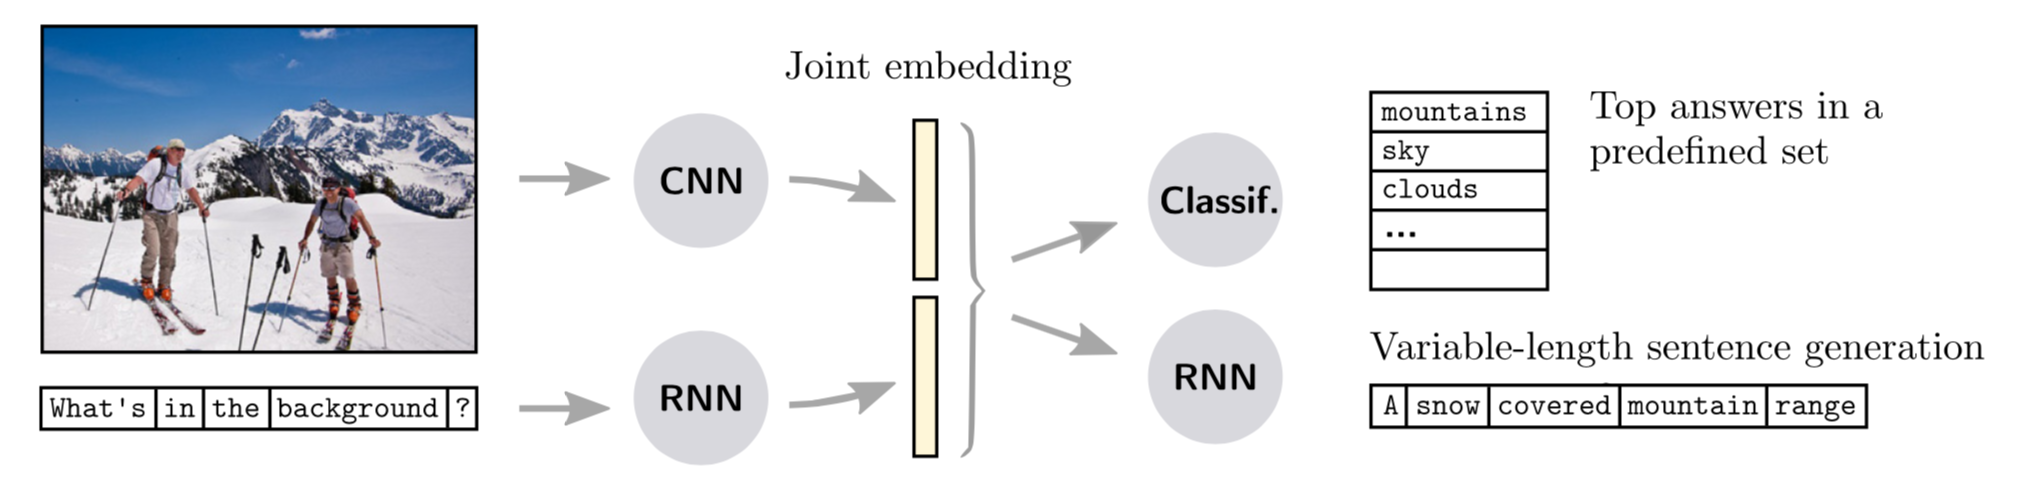
\includegraphics[width=0.8\textwidth]{answer-generation.png}
	\caption{常见的VQA方法是将图像和问题文本映射到同一特征空间,再组合融合两者的形成新的特征向量,特征向量作为分类器或者循环神经网络RNN(也可能是长短期记忆LSTM)的输入,输出得到最终的答案}
	\label{answer-generation}
\end{figure}

本节将简要介绍视觉问答方法中的联合嵌入模型、注意力机制以及动态记忆网络,基于知识库的视觉问答方法将在第二章着重讨论。

\subsection{联合嵌入模型}
联合嵌入模型先将视觉信息和问题文本信息分别特征化,再通过特征向量串联\citing{zhou2015simple}、卷积\citing{ma2016learning}、逐元素相乘\citing{antol2015vqa}、逐元素相加\citing{malinowski2015ask}等池化方法融合图像特征和文本特征,最终得到最优答案。自从深度神经网络在计算机视觉和自然语言处理上的广泛应用以来,将各种模态的信息映射成特征向量的思想便大行其道,因此作为交叉领域中的视觉问答任务自然将多模信息联合嵌入到特征空间视为最“本能”的探索路径。

Malinowski等人首次提出了应用于真实场景视觉问答任务的联合嵌入模型Neural-Image-QA
\citing{malinowski2015ask}。Neural-Image-QA是一个由卷积神经网络CNN和长短期记忆LSTM组成的深度网络,先使用在ImageNet预处理过的卷积神经网络CNN对图像进行特征提取,得到的特征向量和问题文本一起传输到长短期记忆LSTM中,从而生成答案的单词序列。模型在DAQUAR数据集上完成训练和测试,对于答案只有一个词语的问题,准确率为19.43\%,对于答案是多个词语的问题,准确率为17.49\%。

Gao等人提出了mQA模型用于解决视觉问答任务\citing{NIPS2015_5641},mQA由四个部分构成,用于提取问题特征的长短期记忆LSTM(Q)、用于提取视觉特征的卷积神经网络CNN、用于存储具有多词的答案的语义上文的长短期记忆LSTM(A)、用于融合问题特征和已有的部分答案的语义特征并且预测答案的下一个词语的部分。提取视觉特征的CNN采用在ImageNet分类任务上预处理的卷积神经网络,在训练过程中保持不变,训练其他三个部分,以达到最高的准确率。区别于Malinowski的Neural-Image-QA,mQA认为问题和答案在句法结构上有所不同,因此编码问题的LSTM和解码答案的LSTM为采用两个独立的网络,使用不用的权重矩阵,为了降低系统过拟合的风险,共享了词嵌入层。整体架构如图\ref{mQA}。
\begin{figure}[H]
	\centering
	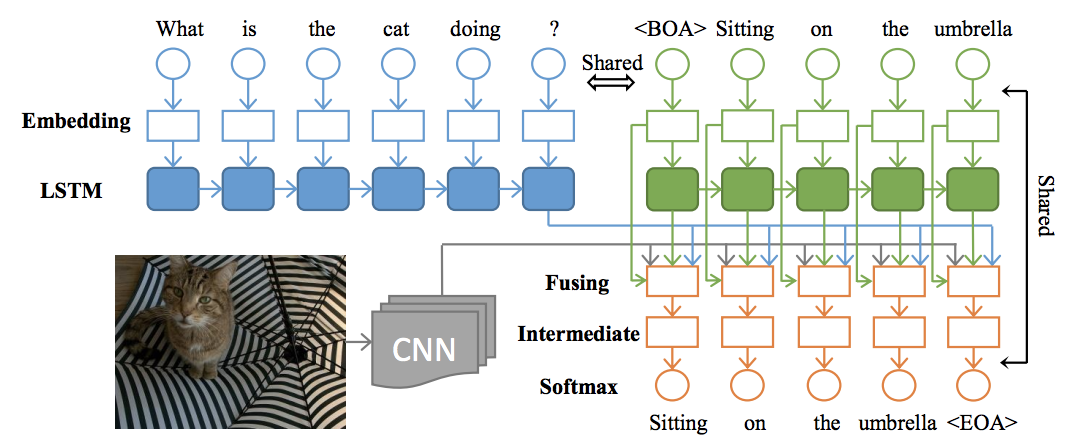
\includegraphics[width=0.8\textwidth]{mQA.png}
	\caption{mQA采用两个独立的LSTM编码问题序列和解码答案序列}
	\label{mQA}
\end{figure}

Noh等人认为单单使用相同权重参数的深度卷积神经网络去处理不同的问题,并期待能得到足够准确的答案,这是很困难的\citing{noh2016image}。因此他们提出DPPnet,在卷积神经网络CNN中添加一个动态参数层,动态参数层中的参数会根据问题的不同而改变,这使得每个问题输入都对应一个独特的分类网络。模型由三个部分组成,一个部分作为分类网络的卷积神经网络,第二个部分是参数预测网络,由门控复发单位编码问题序列,再通过一个全连接层输入动态参数,第三个部分是一个哈希函数,将参数预测网络输出的动态参数配置到分类网络中。如图\ref{DP-CNN}。
\begin{figure}[H]
	\centering
	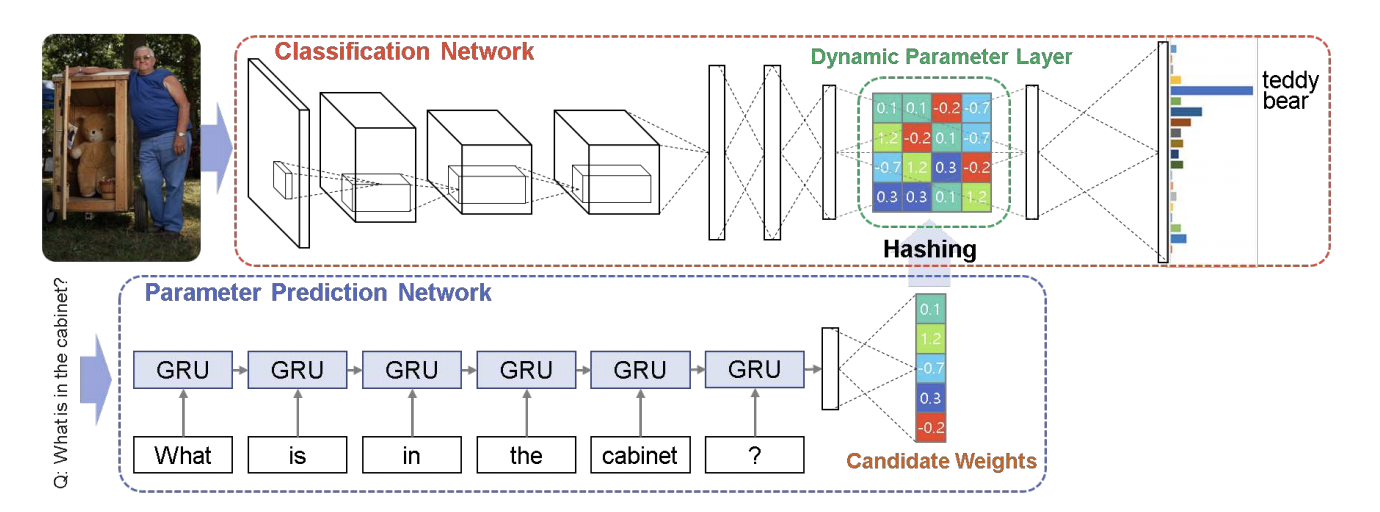
\includegraphics[width=0.8\textwidth]{DP-CNN.png}
	\caption{带有动态参数层的卷积网络模型DPPnet}
	\label{DP-CNN}
\end{figure}

Zhou等人同样适用预处理后的卷积神经网络CNN,但在处理问题文本时选择了比长短期记忆LSTM更为简单的词袋模型BOW,提出了iBOWIMG模型\citing{zhou2015simple}。iBOWIMG模型受到BOWIMG\citing{antol2015vqa}在VQA数据集上优于部分基于长短期记忆LSTM模型的启发,在原有基础上将VGGNet替换为在图像特征提取表现更优的GoogLeNet\citing{Szegedy_2015_CVPR},将图像特征向量和文本特征向量串联后送入softmax层预测问题答案(如图\ref{iBOWIMG}),在COCO-VQA数据集上的测试展现出具有竞争力的表现。
\begin{figure}[H]
	\centering
	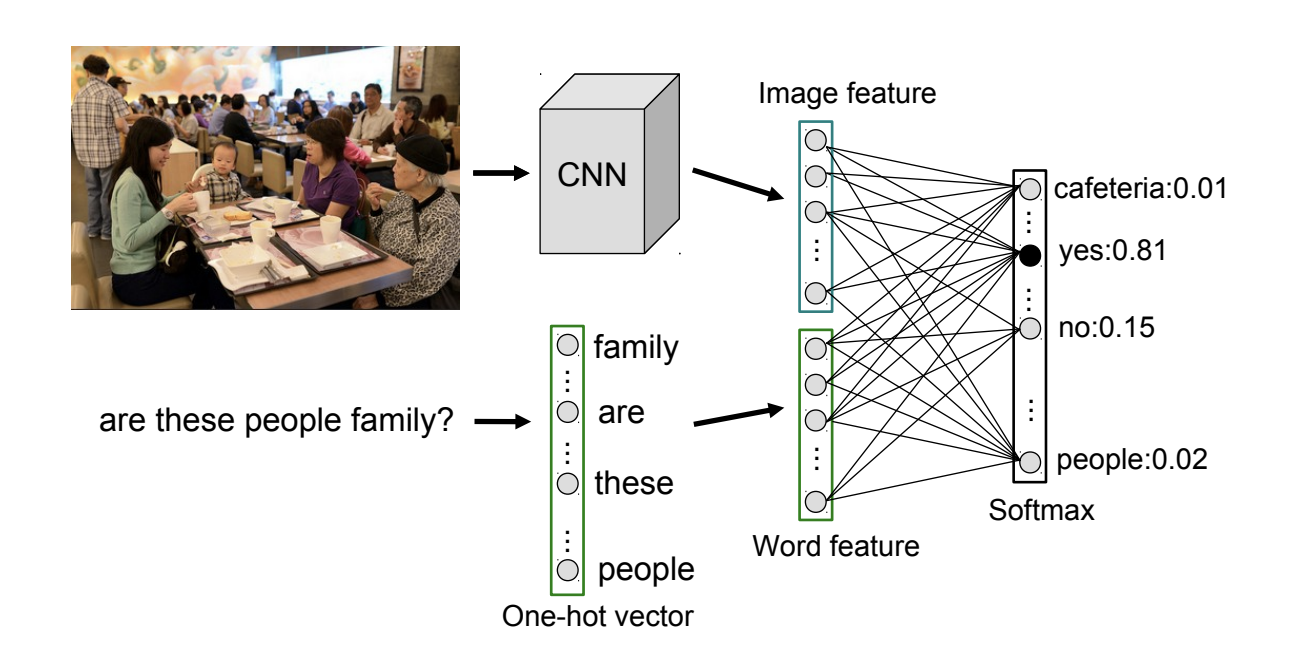
\includegraphics[width=0.8\textwidth]{iBOWIMG.png}
	\caption{iBOWIMG使用词袋BOW模型作为词特征向量编码器}
	\label{iBOWIMG}
\end{figure}

Lin等人将卷积神经网络CNN不仅应用于编码图像内容,而且也应用于问题文本的提取\citing{ma2016learning}。在处理图像特征和文本特征时使用一个多模态的卷积层输出联合特征向量,再使用softmax层预测最终的答案。如图\ref{lin}。
\begin{figure}[H]
	\centering
	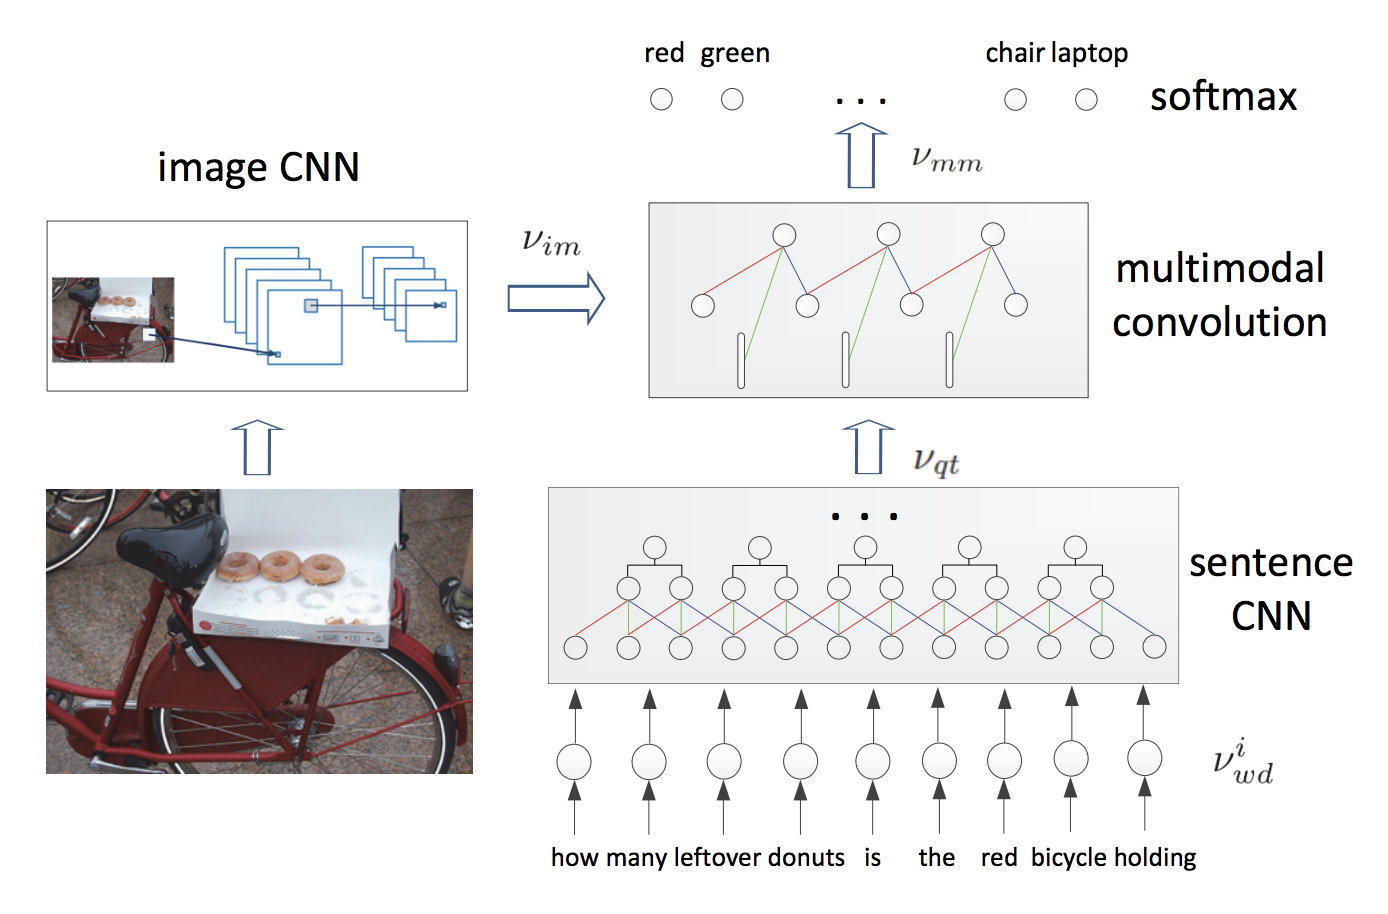
\includegraphics[width=0.8\textwidth]{lin.png}
	\caption{图像特征和问题文本特征提取时均使用CNN}
	\label{lin}
\end{figure}

除了使用不同的方法提取图像和文本特征以外,联合嵌入模型的另一个能够显著改善模型准确率的方向就是实验不用特征向量融合的池化方法。Malinowski等人通过对不同的特征向量融合方法的比较,可以看出系统的准确率与特征向量融合方法有关,不同方法之间准确率最多能相差9个百分点之多\citing{malinowski2015ask}。除了以上提到的iBOWIMG采用向量串联的方式,Lin使用向量卷积的方式外,Antol等人提出的模型使用逐元素相乘的方法融合两者\citing{antol2015vqa},Saito等人认为不同的特征融合方法各有特点,会保留或损失不同的特征,为了充分利用不同方法所保留的特征,提出了一种融合逐元素相加和逐元素相乘相结合的模型DualNet。模型同样利用了使用不同卷积神经网络CNN提取的图像特征,例如在真实场景图像采用了VGG-19\citing{simonyan2014very}、ResNet-152和ResNet-101\citing{he2016deep}。DualNet对提取出的文本特征和图像特征分别使用逐元素相加和逐元素相乘的方法得到两个不同的联合向量,再将两个的联合向量串联得到最终的合成向量,如图\ref{DualNet}。
\begin{figure}[H]
	\centering
	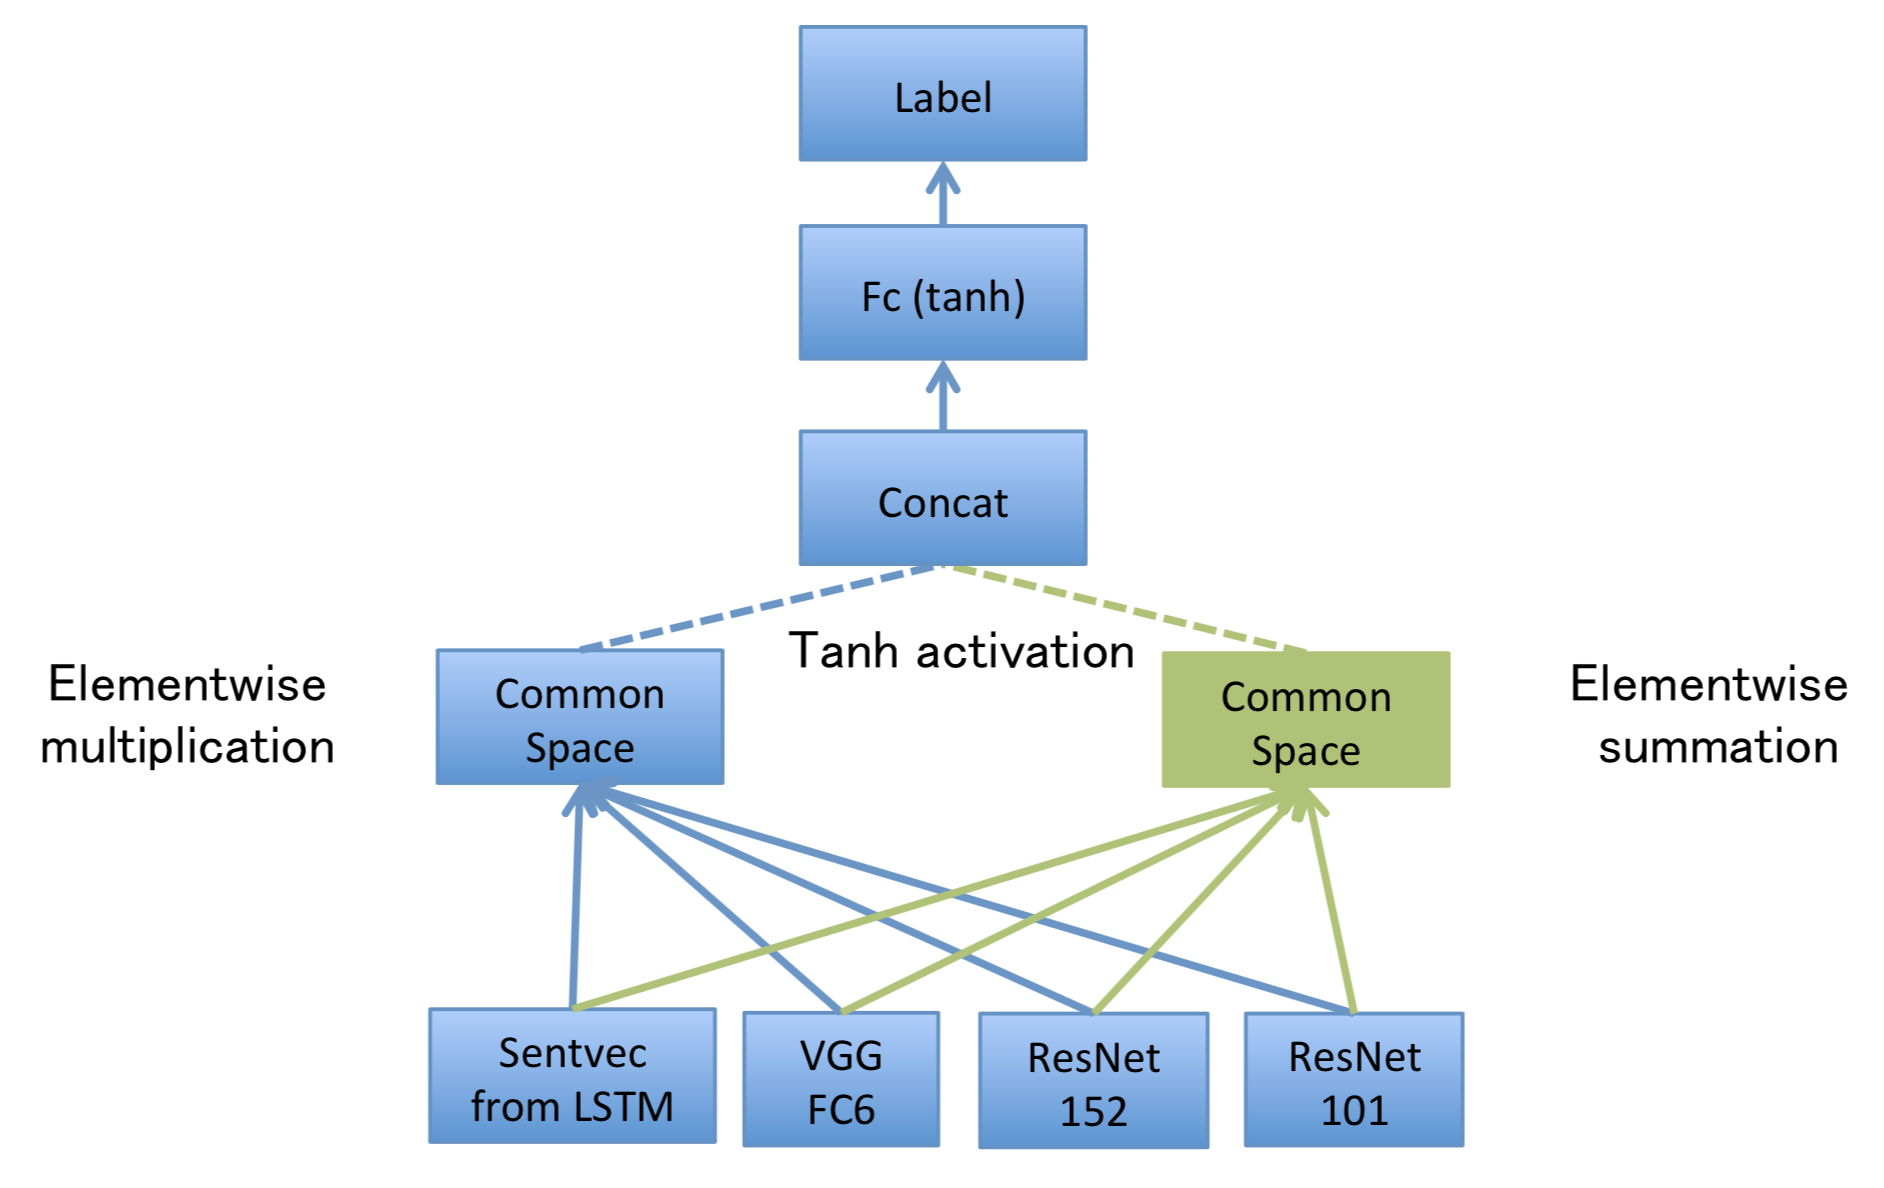
\includegraphics[width=0.8\textwidth]{DualNet.png}
	\caption{DualNet针对真实场景图像的模型架构}
	\label{DualNet}
\end{figure}

Fukui等人认为向量之间的外乘运算中,所有元素之间的互动更加活跃,应该能保留更加丰富的特征信息,因此提出一种更为复杂的多模态紧凑双线性池化方法(MCB)。一般的双线性模型会对两个向量的外乘结果线性化,外乘操作会得到异常高维的向量,例如外乘的两个向量维度均为2048、输出向量维度为3000时,那么训练参数的数量将达到125亿个之多,这会导致巨大的计算开销。而提出的多模态紧凑双线性方法能避免直接计算向量外乘,同时保留了大量特征,模型架构如图\ref{mcb}。
\begin{figure}[H]
	\centering
	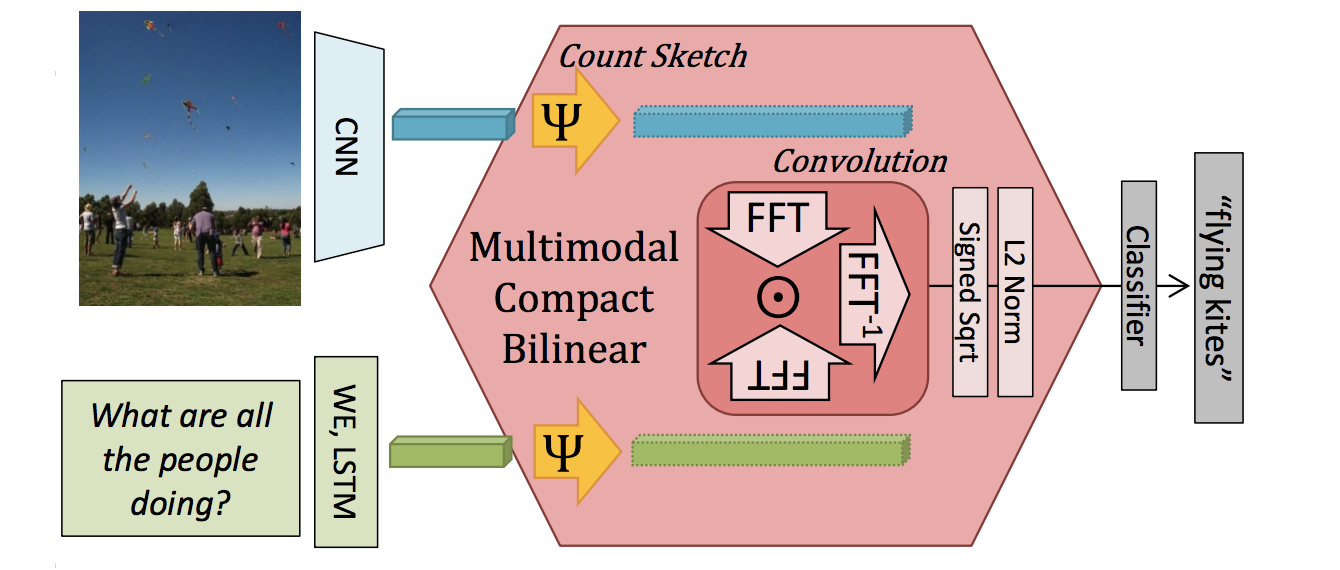
\includegraphics[width=0.8\textwidth]{mcb.png}
	\caption{使用多模态紧凑双线性池化融合图像和文本特征}
	\label{mcb}
\end{figure}

\subsection{注意力机制}
人类获取外部视觉信息时,会自动形成一种“像素不均衡”,在同一视野范围内的像素被视觉中枢神经系统根据“关注区域”的远近、相关性特征自动分配不同的分辨率,使得“关注区域”内的像素具有极高的分辨率,而其他的像素仅仅作为视觉信息输入,并不参与大脑的语义处理(如图所示\ref{human-virtual})。因此视觉注意力机制帮助大脑过滤了低相关性的视觉信息,减少了待处理数据的体积,极大地提高了信息处理速率并松弛了大脑负载。
\begin{figure}[H]
	\centering
	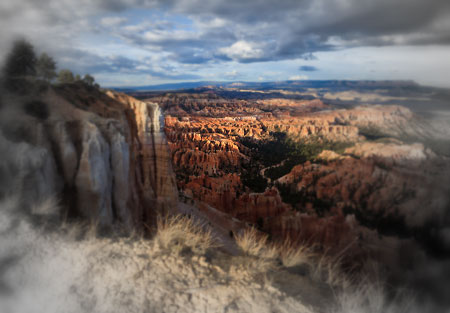
\includegraphics[width=0.5\textwidth]{human-virtual.png}
	\caption{人类视觉系统的“像素不均匀”现象}
	\label{human-virtual}
\end{figure}

近几年,受到人类视觉注意力机制的启发,在神经网络中引入注意力机制变得十分热门,在自然语言处理和计算机视觉领域的应用也极大得帮助了原有算法精度和计算效率的提升。Google Deepmind团队提出了一种带有注意力机制的循环神经网络(RNN),并成功应用于图像分类任务,获得了优于以往卷积神经网络(CNN)的基线水平的分类精度\citing{mnih2014recurrent}。随后,带有注意力机制的循环神经网络便被广泛应用于自然语言处理和计算机视觉的多个子领域\citing{bahdanau2014neural, xu2015show, NIPS2015_5847}。Bahdanau等人将注意力机制引入神经机器翻译任务,仍然使用“编码-解码”的翻译模式,但一改以往将源语言文本映射为一个固定长度的向量的编码方式,而是将原语言文本编码为向量序列,解码时将翻译和位置对应因素联合学习,训练向量序列中各向量对翻译词组的不同权重,加和完成翻译结果的推断,得到了以往最优的结果\citing{bahdanau2014neural}。Xu等人受到注意力机制在机器翻译和物体识别任务成功应用的启发,将带有注意力机制的循环神经网络应用于自动生成图片说明,并且在Flickr9k, Flickr30k 和MS COCO 三个数据集上均获得了最优的结果\citing{xu2015show}。随后,更多注意力机制的变型或优化研究均在图片说明任务上展开\citing{ 7243334, wu2017global, li2017image, lu2017knowing}。

相较起图片说明任务,视觉问答任务除了要求系统能理解图片内容,生成语义和句式合理的自然语言文本以外,还需要联合学习问题文本和聚焦与问题相关的图像细节。这些任务特性决定了视觉问答任务可以利用已有较为先进的图片说明任务的框架,同时融合自然语言处理的最新成果。注意力机制在自然语言处理和计算机视觉上的成功应用便成为了视觉问答算法快速发展的基石。

Chen等人最先将注意力机制引入视觉问答任务,提出了基于注意力机制的可配置卷积神经网络(ABC-CNN)用于针对“图像问题对”生成对应的注意力映射,将问题的语义信息和图像区域建立映射,使得答案生成取决于被关注区域,减少无关区域的影响\citing{chen2015abc}(模型架构如图\ref{abc-cnn})。在Toronto COCO-QA\citing{ren2015exploring}, DAQUAR\citing{ malinowski2014multi}, 和VQA\citing{antol2015vqa}三个数据集上的测试结果都提升了最优结果,证明了注意力机制在提高视觉问答任务上的有效性,同时注意力权重图能反应系统的推理过程,为参数的微调提供了依据。
\begin{figure}[H]
	\centering
	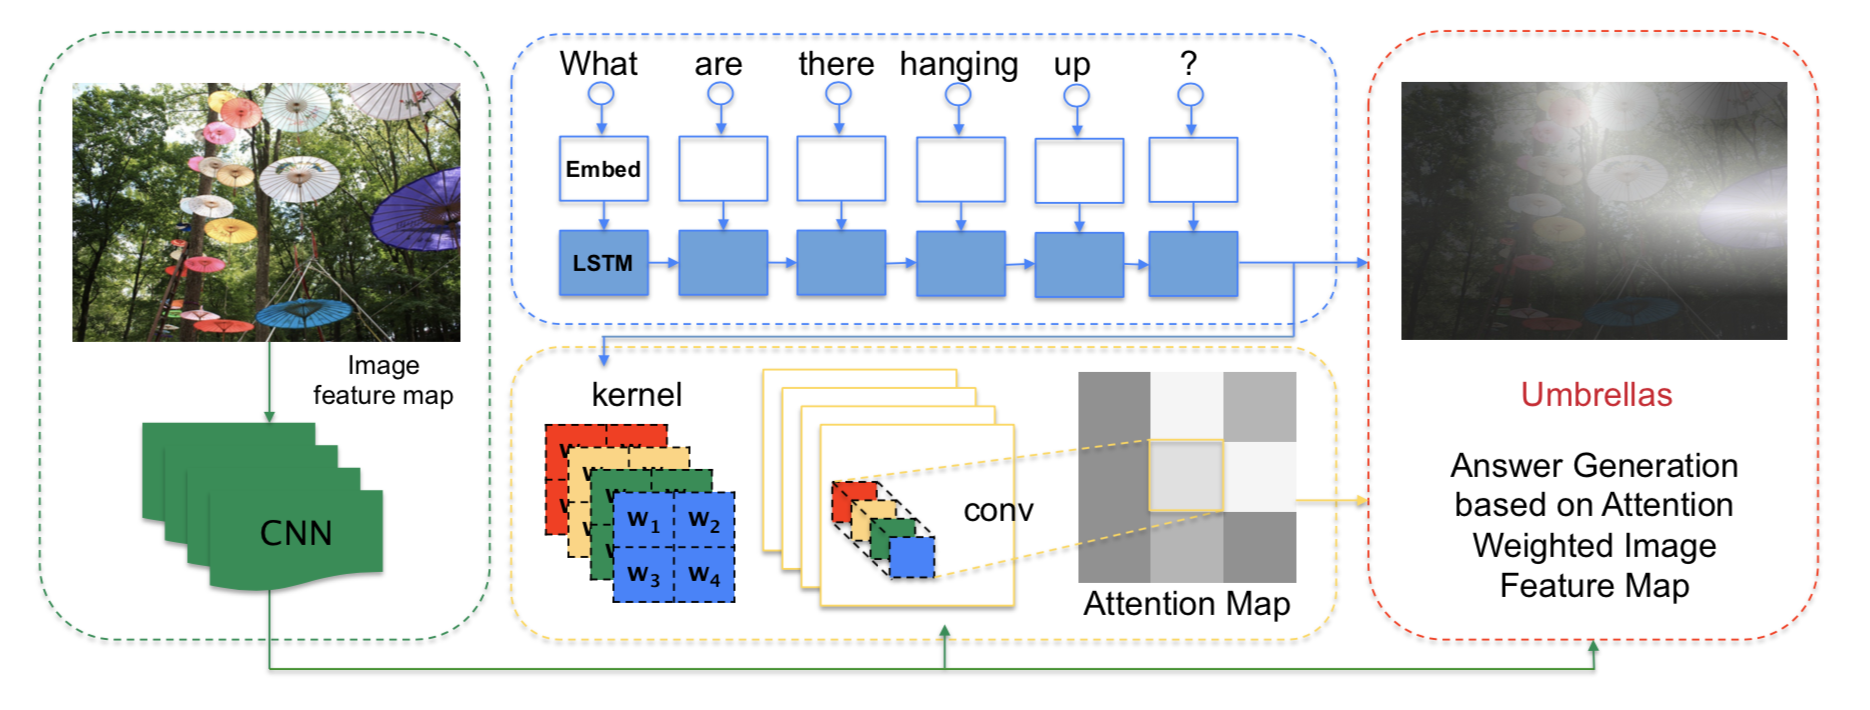
\includegraphics[width=0.8\textwidth]{abc-cnn.png}
	\caption{ABC-CNN使用CNN提取图像特征,LSTM提取问题文本特征,黄色方框内为用于推测与问题相关的图像区域的注意力机制}
	\label{abc-cnn}
\end{figure}

Shih等人使用简单的word2vec方法编码“问题-答案”对,使用预处理后的卷积神经网络CNN对图片的不同区域编码,将编码后的文本特征向量和图片特征向量映射到同一特征空间,根据特征之间的点乘运算决定每个图像区域的权重,最后结合权重化以后的图像特征和文本特征得出答案。架构如图\ref{shih}。在辨别物体颜色的任务上得到了最优结果\citing{ shih2016look}。类似的工作还有Ilievski等人提出的“聚焦型动态注意力模型“\citing{ilievski2016focused}。
\begin{figure}[H]
	\centering
	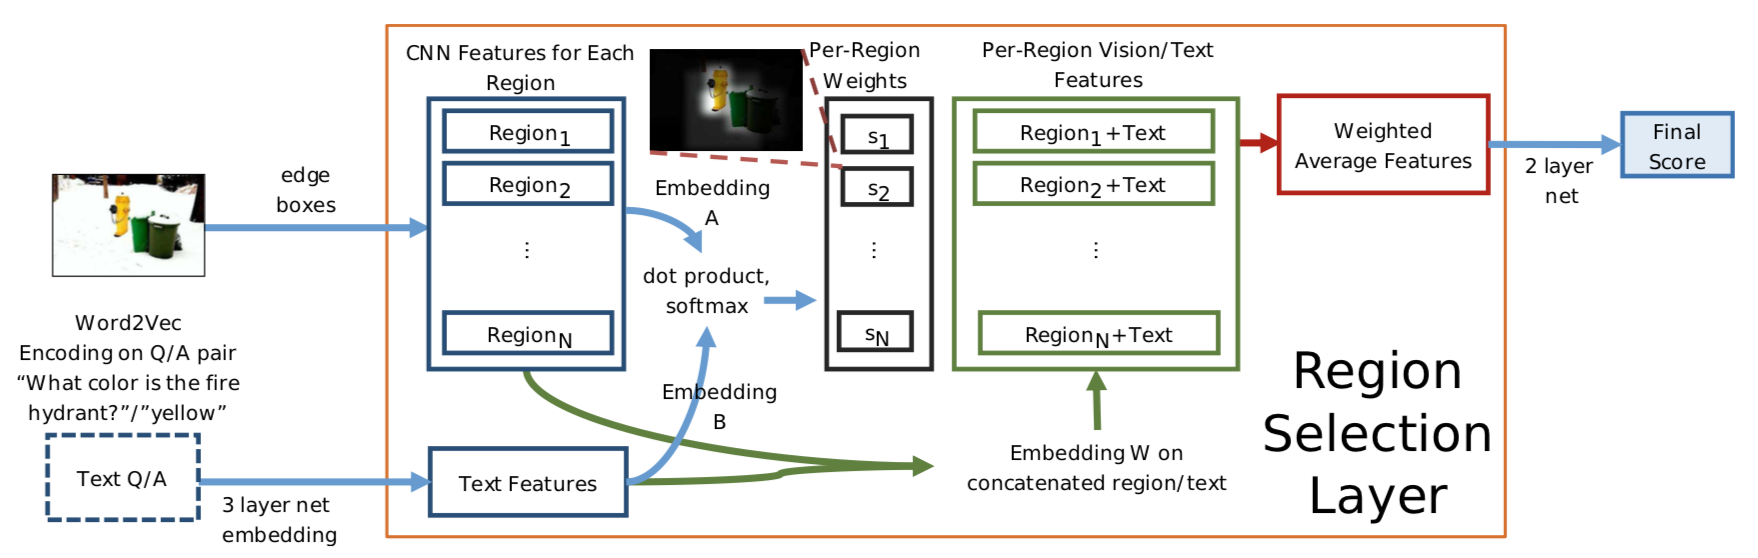
\includegraphics[width=0.8\textwidth]{shih.png}
	\caption{使用图片区域选择层实现注意力机制的架构}
	\label{shih}
\end{figure}

包括以上提到的在内,多数注意力机制对问题文本和图像区域特征进行一次运算,直接生成图像注意力权重图。针对这种情况,Yang等人提出堆栈式注意力网络——使用问题的语义表达对图像进行多次查询,不断缩小答案相关区域,实现更高的精度\citing{yang2016stacked}。注意力机制在视觉问答上的其他应用还有,同时使用对图像和问题使用注意力机制的联合注意力模型\citing{NIPS2016_6202};不采用图像区域赋值方法,而是过滤掉不相关区域的“自适应硬性注意力网络”\citing{malinowski2018learning}。

对于神经网络训练这类参数密集和计算密集的框架,注意力机制能带来两个重要的改变。一方面,无论对于图像输入还是文本输入,原有的方法都选择将输入看做一个整体,因此映射后的向量需要包含完整的输入信息,对于包含词组过多文本或是场景过于复杂的图像,编码后的向量根本无法区分开输入的局部特征,这使得神经网络的可解释性大大降低。引入注意力机制后,编码方式改变,将输入视为为局部信息的综合,保留了文本中单词和图像中像素区域的信息,通过可视化处理,能清晰的看出神经网络的推理过程,增强了系统的可解释性,可以称之为一种“弱化黑盒的处理”。另一方面,注意力机制非常符合人类对于语言和视觉信息的处理方式,这背后的假设是:针对绝大多数任务,只需要从信息源的局部便能获得充分正确的答案。类似于人类,具有注意力机制的智能体应当能获得更高的执行的效率和更高的答案精度。

\subsection{动态记忆网络}
无论是在自然语言理解还是图像内容理解,人类在获取单词或者图像像素区域的语义时不会将其与语境割裂来看,通常上下文语境对于准确理解文本和图像信息是非常重要的,因为在语言和图像中存在大量具有歧义特性的内容,例如,在语言中一个单词具有不同的语义,也可能有不同的词性,只有在上下文的语境中才能确定词语的真正含义。记忆力与上下文语境相似,是神经网络在训练过程中存储的“经验”,这种“经验”有助于以后的训练,这种累积经验能创造更准确的答案,基于这样的假设,研究人员为从序列化的输入中获得更准确的输入,而引入了动态记忆网络\citing{jiang2015compositional,kumar2016ask,xiong2016dynamic}。

Jiang等人在常见的CNN解析图像、LSTM解析问题文本的架构上,新增一个成分记忆模块\citing{jiang2015compositional},旨在融合每一次训练过程中的局部图像信息和文本信息,并提供给下一次训练使用,从而使网络存储了训练过程的“经验”,这与之后提出的动态记忆网络有同样的思想,模型训练流程如图\ref{c-memory}。
\begin{figure}[H]
	\centering
	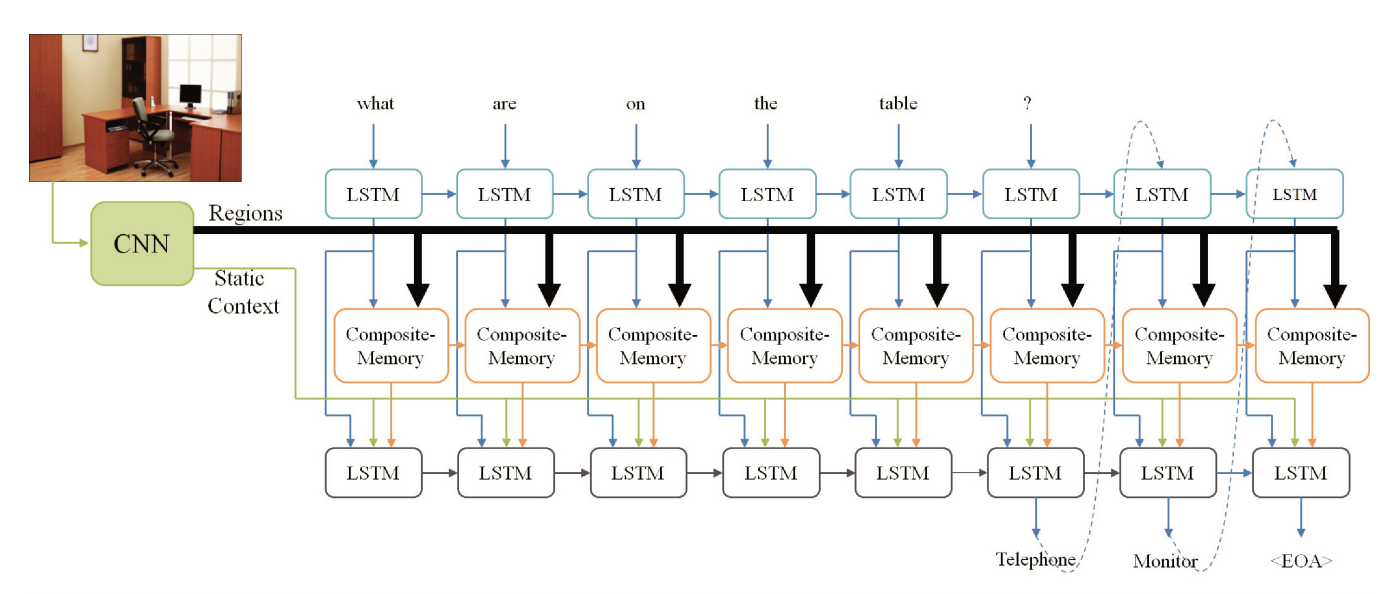
\includegraphics[width=0.8\textwidth]{c-memory.png}
	\caption{成分记忆模型的训练流程}
	\label{c-memory}
\end{figure}

Kumar等人为解决文本问答(Text-QA)任务而提出动态记忆网络(DMN)\citing{kumar2016ask}。动态记忆网络(DMN)是一个用于生成文本问题答案的神经网络框架,它由输入模块、问题模块、情节记忆模块和问题模块构成,输入模块用于编码文本输入;问题模块用于编码文本问题;情节记忆模块接受由输入和问题模块得到的分布式向量,再使用注意力机制选择部分接受到的向量,结合选择后的向量与以往存储的“记忆”生成新的“记忆”向量,并不断迭代;答案模块根据最终的记忆向量生成答案,模型架构如图\ref{dmn}。
\begin{figure}[H]
	\centering
	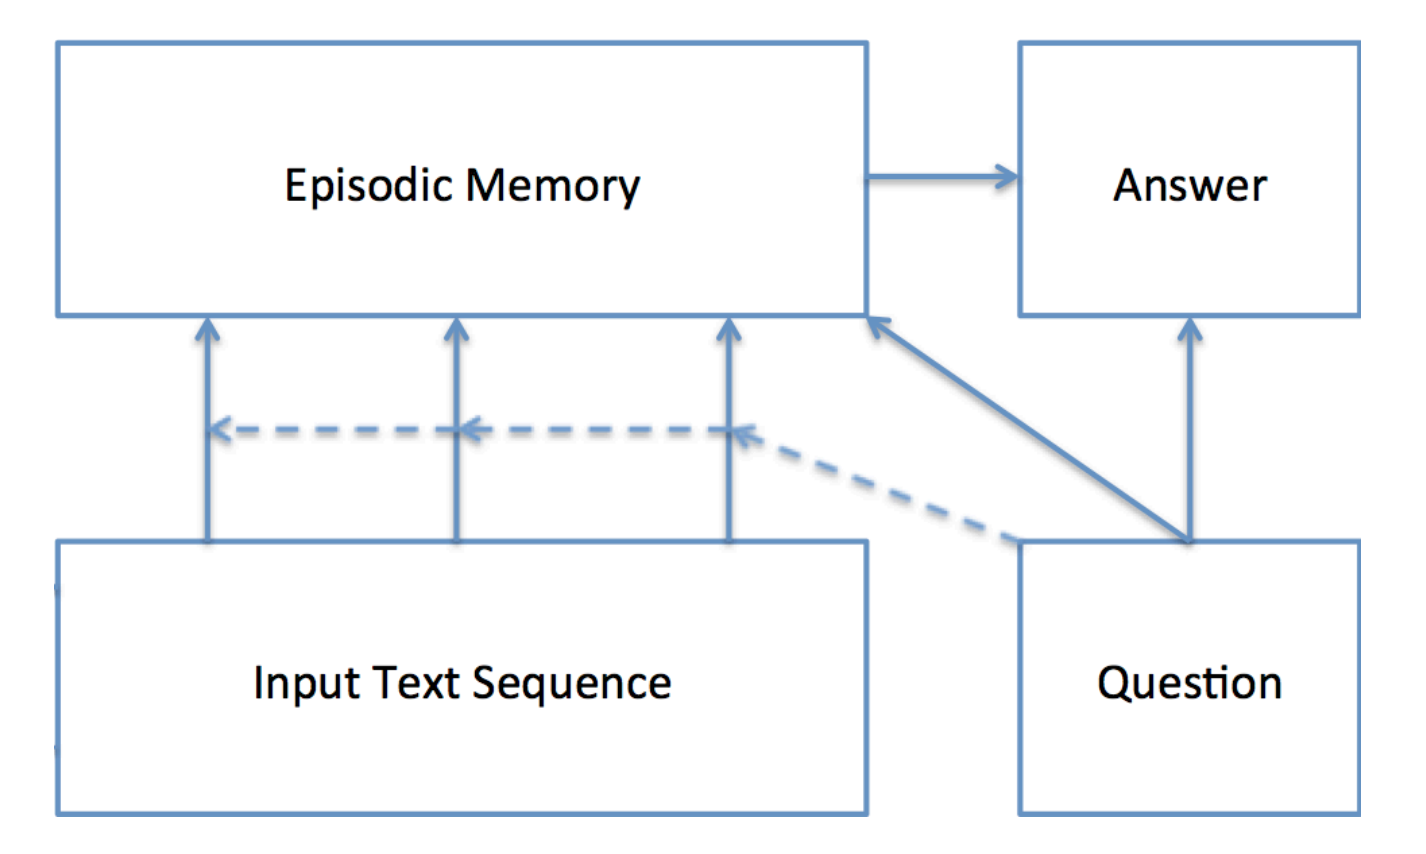
\includegraphics[width=0.5\textwidth]{dmn.png}
	\caption{DMN基础架构}
	\label{dmn}
\end{figure}

动态记忆网络(DMN)在文本问答、语义分析、词性标注任务上取得了最优的结果,受到其在处理序列化的文本信息上的优异表现的启发,Xiong等人在原有网络的基础上改善了输入和记忆模块,除了能处理文本信息外,还能处理图像信息,提出应用到于视觉问答任务动态记忆网络+(DMN+)\citing{xiong2016dynamic},如图\ref{v-dmn}。动态记忆网络+(DMN+)将原有的输入模块中处理文本编码的门控复发单元(GRU)更换为双向门控复发单元(bi-GRU)以得到文本或图像区域更完整的上下文信息;使用基于注意力机制的门控复发单元替换原有的软性注意力机制。更新后的动态记忆网络+(DMN+)在DAQUAR\citing{malinowski2014multi}和VQA数据集\citing{antol2015vqa}上的测试结果都得到了具有竞争力的表现。
\begin{figure}[H]
	\centering
	\subfigure[应用于文本问答的动态记忆网络(DMN)模型架构]{
		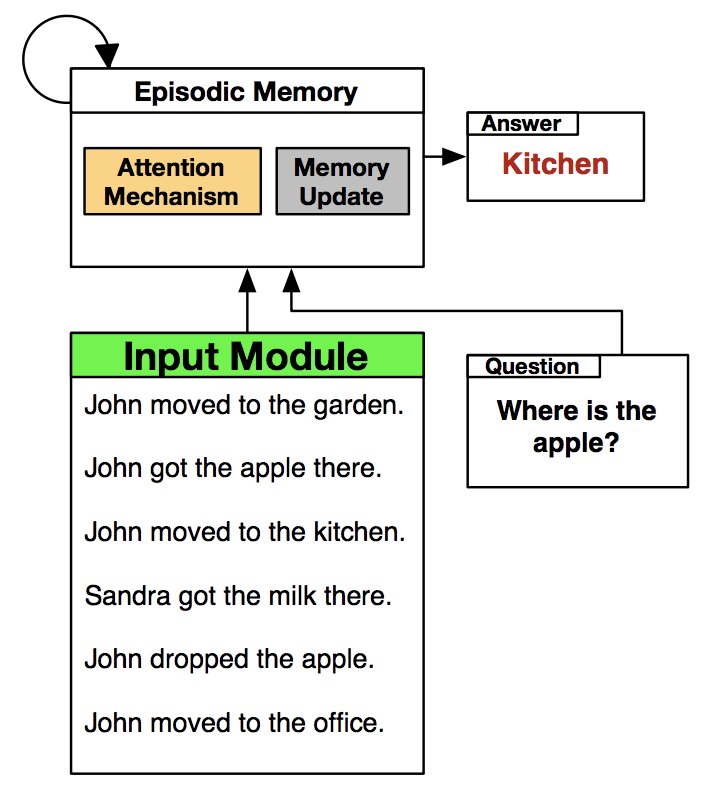
\includegraphics[width=0.4\textwidth]{t-dmn.png}}
	\subfigure[应用于视觉问答的动态记忆网络+(DMN+)模型架构]{
		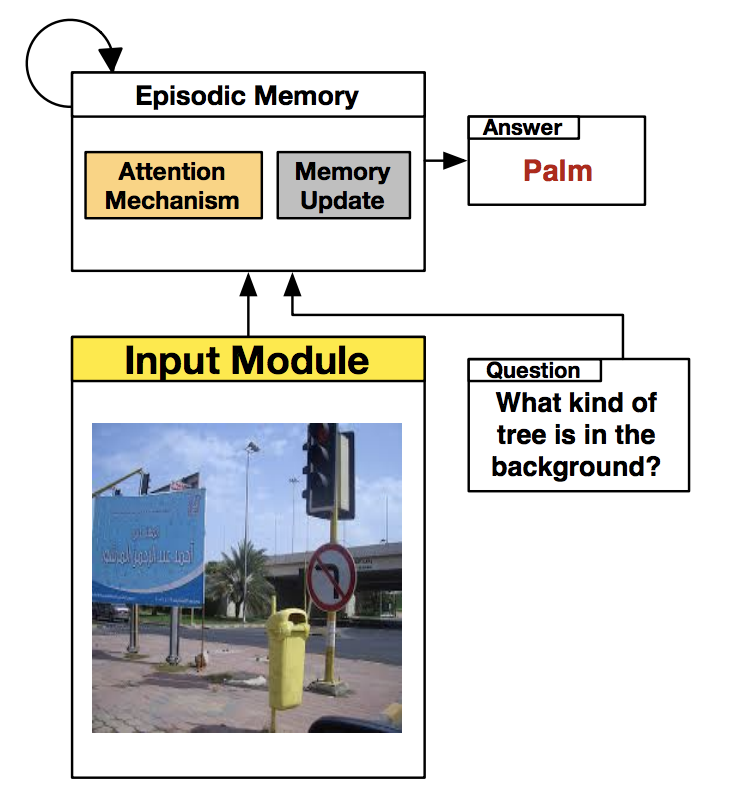
\includegraphics[width=0.4\textwidth]{v-dmn.png}}
	\caption{DMN+与DMN架构对比}
	\label{v-dmn}
\end{figure}

\section{本文的主要贡献与创新}
本论文以时域积分方程时间步进算法的数值实现技术、后时稳定性问题以及两层平面波加速算法为重点研究内容,主要创新点与贡献如下:

\section{本论文的结构安排}
本文的章节结构安排如下:
